\documentclass[x11names]{article}
\usepackage{tikz}
\usepackage{pgfplots}
\usepackage{xcolor}
\usepackage{svg}
\usepackage{amsmath}
\usepackage{array}
\usepackage[skins]{tcolorbox}
\usepackage[version=4]{mhchem}
\usepackage[a4paper, total={6in, 10in}]{geometry}
\usepackage{fourier}
\usepackage{xymtex}
\usepackage{textcomp}
\usepackage{eurosym}
\usepackage{mathrsfs}
\usepackage{float}
\usepackage{pst-all}
\usepackage{pst-3dplot}
\usepackage{leftindex}
\usepackage{verbatim}
\usepackage{import}
\usepackage{xifthen}
\usepackage{pdfpages}
\usepackage{transparent}
\usepackage{import}
\usepackage{pdfpages}
\usepackage{transparent}
\usepackage{amssymb}
\usepackage{mathrsfs}
\usepackage{hyperref}


\definecolor{myblue}{RGB}{224, 245, 255} 
\definecolor{myred}{RGB}{234, 222, 255}



% box
\newtcolorbox{es}[2][]{%
  enhanced,colback=white,colframe=black,coltitle=black,
  sharp corners,boxrule=0.4pt,
  fonttitle=\itshape,
  attach boxed title to top left={yshift=-0.5\baselineskip-0.4pt,xshift=2mm},
  boxed title style={tile,size=minimal,left=0.5mm,right=0.5mm,
    colback=white,before upper=\strut},
  title=#2,#1
}

% definizioni
\newtcolorbox{blues}[2][]{%
  enhanced,colback=myblue,colframe=black,coltitle=black,
  sharp corners,boxrule=0.4pt,
  attach boxed title to top left={yshift=-0.5\baselineskip-0.4pt,xshift=2mm},
  boxed title style={tile,size=minimal,left=0.5mm,right=0.5mm,
    colback=myblue,before upper=\strut},
  title=#2,#1
}

% teoremi
\newtcolorbox{redes}[2][]{%
  enhanced,colback=myred,colframe=black,coltitle=black,
  sharp corners,boxrule=0.4pt,
  fonttitle=\itshape,
  attach boxed title to top left={yshift=-0.5\baselineskip-0.4pt,xshift=2mm},
  boxed title style={tile,size=minimal,left=0.5mm,right=0.5mm,
    colback=myred,before upper=\strut},
  title=#2,#1
}


% comandi per quadrati dimostrazioni
\newcommand*{\QEDA}{\null\nobreak\hfill\ensuremath{\blacksquare}}%
\newcommand*{\QEDB}{\null\nobreak\hfill\ensuremath{\square}}%


%% regole
\renewcommand*\contentsname{Indice}
\setcounter{tocdepth}{3}
\setcounter{secnumdepth}{2}
\pgfplotsset{compat=1.15}

\usetikzlibrary{arrows}


\title{Geometria e Algebra lineare}
\author{Federico Cesari}
\date{}



%% DOCUMENTO


\begin{document}

\begin{titlepage}
	\begin{center}
		\vspace*{1cm}
		
		\textbf{\LARGE Relazione di laboratorio - Pendolo semplice}
		
		\vspace{0.3cm}
		\large \textit{Misura del periodo di un pendolo semplice} \\
		
		\vspace{0.5cm}
		\Large Federico Cesari \\
		
		\small 1096759 
		\vspace{0.2cm}
		
		\small Gruppo 5
		
		
		\vspace{3cm}
		\begin{center}
			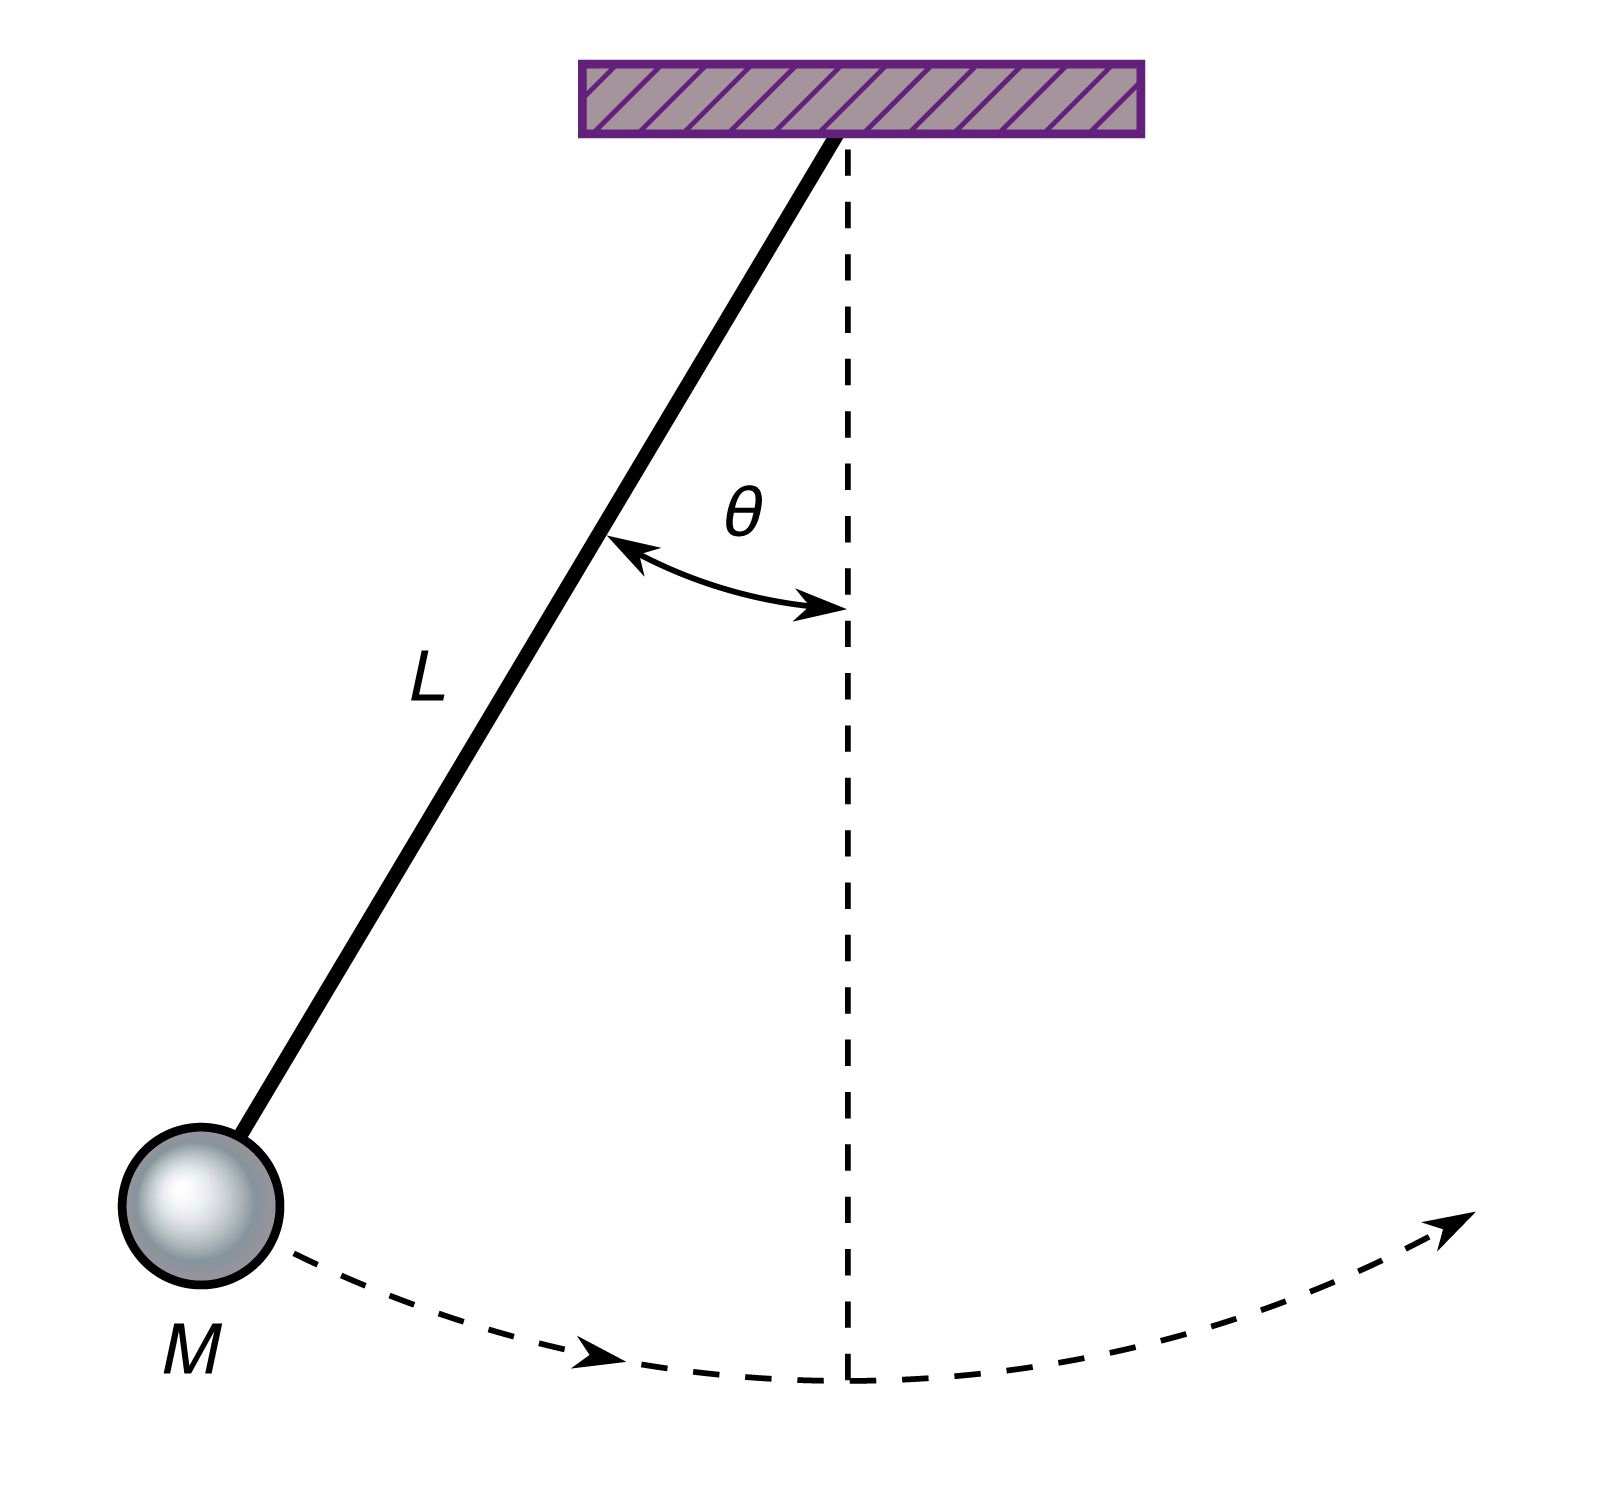
\includegraphics[scale=0.1]{IMG_0200.jpeg}	
		\end{center}
		
		
		
		\vfill
		
		
		
		corso A\\
		Università degli studi di Torino, Torino\\
		4 aprile 2024\\
		
		
	\end{center}
\end{titlepage}
\tableofcontents
\newpage







%% %% %%
%% %% %%  Sistemi di equazioni lineari
%% %% %% 

\newpage
\section{Sistemi di equazioni lineari}
 Prima di parlare di sistemi definiamo cosa si intende per \textit{equazione lineare}: un'equazione lineare è un'uguaglianza del tipo  
 $$a_{1}x_{1} + a_{2}x_{2}... a_nx_n=b$$ 

 espressa nelle incognite $x_1$, $x_2$,... $x_n$. Un'equazinone di questo genere ha come soluzione una n-upla di numeri reali che sostituiti al posto delle incognite rende vera l'uguaglianza (la \textit{risoluzione} dell'equazione consiste nel trovare questa n-upla).

 \begin{es}{esempio}
     Definiamo un'equazione $*$ 
     $*:x_1 - x_2 + 2x_3 = 4 \qquad \textnormal{con} \qquad x_1 = x_2 - 2x_3 + 4$  \\
     L'insieme delle soluzioni di $*$ lo indichiamo con $S_{(*)}$ 
      $S_{(*)} = \Biggl\{\begin{pmatrix}x_2 - 2x_3 + 4 x_2  x_3 \end{pmatrix}: x_2, x_3 \in \mathbb{R}\Biggl\} $ 
      In cui $x_2$ e $x_3$ sono i parametri liberi che variano.
 \end{es}

 \begin{es}{esempio}
     Utilizzando un'altra equazione $*$ 
     $*: 2x - 3y = 0$  \\
     L'insieme delle sue soluzioni sarà: 
     $S_{(*)} = \Biggl\{\begin{pmatrix}x  y \end{pmatrix}: x,y \in \mathbb{R}\Biggl\} $ 
     oppure tramite un parametro $t$ per il quale $\begin{cases}x=ty=\frac{2}{3}t ,\quad t \in \mathbb{R}\end{cases}$ 
      $S_{(*)} = \biggl\{(t,\frac{2}{3}t): t \in \mathbb{R}\biggl\} $
 \end{es}

 \vspace{2em}
 Definiamo invece un \textit{sistema lineare} di $r$ equazioni lineari in $n$ incognite $x_1, x_2 \dots x_n$ una struttura del tipo:

 $$ 
 {\begin{cases}a_{11}x_{1}+a_{12}x_{2}+\cdots +a_{1n}x_{n}=b_{1}\\a_{2,1}x_{1}+a_{22}x_{2}+\cdots +a_{2n}x_{n}=b_{2}\\\vdots a_{r1}x_{1}+a_{r2}x_{2}+\cdots +a_{rn}x_{n}=b_{r}\end{cases}} 
 $$
 i coefficienti sono espressi nella forma $a_{ij}$ per agevolarne il riconoscimento all'interno del sistema. Il  pedice $i$ indica l'indice di riga, il pedice $j$ è l'indice di colonna. I termini noti $b$ presentandosi una sola volta per riga hanno solo l'indice di riga.
 Se i termini noti sono tutti nulli il sistema si dirà \textbf{\textit{omogeneo}}

 Diremo soluzione del sistema una n-upla di numeri reali $\begin{pmatrix}x_{1}\\ \vdots \\ x_{n}\end{pmatrix}$ che risolve ciascuna delle equazioni del sistema. Il sistema si dice \textbf{\textit{compatibile}} se ammette soluzioni (altrimenti \textbf{\textit{incompatibile}}).  Due sistemi sono \textbf{\textit{equivalenti}} se hanno lo stesso insieme di soluzioni. 
 
\begin{center}
\includesvg[scale=0.6]{figures/sistemi_piani}
\end{center}

\begin{center}
\fboxsep11pt
\colorbox{myred}{\begin{minipage}{5.75in}
\begin{redes}{Teorema di Rouchè-Capelli}
%ROUCHE CAPELLI
Un sistema lineare $AX = B$  con $A \in \mathbb{R}^{r,n}, \quad X \in \mathbb{R}^{n,p}, \quad B \in \mathbb{R}^{r,p}$ è compatibile se e solo se il rango della matrice
dei coefficienti coincide con il rango della matrice completa. Se il sistema è compatibile, le soluzioni dipendono da $p \cdot \left(n-\text{rk}A\right)$ parametri liberi.
\[
	\text{rk}\left(A|\overline{b}\right) = \text{rk}\left(A\right) \quad \Rightarrow \quad \text{sistema compatibile}
\] 
\end{redes}
\end{minipage}}        
\end{center}

Poiché si opera solo sui coefficienti e non sulle incognite, i calcoli su essi risultano facilitati tramite l'utilizzo di tabelle (matrici). Un sistema quindi, nella sua forma matriciale (completa perché contiene anche i termini noti) il sistema si presenta così:

\[
\left(A|\overline{b}\right)=
\left(\begin{array}{ccc|c}
a_{1,1}&\cdots &a_{1,n}&b_{1} \\ \vdots &\ddots &\vdots  &\vdots \\ a_{r,1}&\cdots &a_{r,n}&b_{r}
\end{array}\right)
\] 

In questa forma la matrice è scomponibile e riscrivibile come il prodotto scalare tra il vettore dei coefficienti $\overline{a}$ e il vettore delle incognite $\overline{x}$:

\[
\begin{pmatrix}
a_{11}&a_{12}&\cdots &a_{1n}\\
a_{21}&a_{22}&\cdots &a_{2n}\\
\vdots &\vdots &\ddots &\vdots\\ 
a_{r1}&a_{r2}&\cdots &a_{rn}
\end{pmatrix}
\begin{pmatrix}x_{1}x_{2}\\
\vdots x_{n}
\end{pmatrix}=
\begin{pmatrix}
b_{1} \\
b_{2} \\
\vdots\\ 
b_{r}
\end{pmatrix}
\]

%OMOGENEO
\subsection{Sistemi omogenei}
Particolarità dei sistemi omogenei è il fatto che operando sulle righe, non si va ad alterare sulla colonna di zeri. Ogni sistema omogeneo ricade in due possibili scenari:

\begin{enumerate}
 	\item Ha solo la soluzione banale;
	 \item Ha altre infinite soluzioni oltre quella banale.
\end{enumerate}


\begin{center}
\fboxsep11pt
\colorbox{myred}{\begin{minipage}{5.75in}
\begin{redes}{Teorema: parametri liberi}
Se un sistema lineare omogeneo ha $n$ incognite e nell sua forma ridotta la sua matrice completa ha  $\text{rank}A = n$ (nessuna riga nulla), allora
\[
\text{parametri liberi } = n - \text{rank}A
.\] 
\end{redes}
\end{minipage}}        
\end{center}

 

%SISTEMA OMOGENEO ASSOCIATO
\noindent
Se conosco una soluzione $x_0$ di $\Sigma$, sommandoci una qualsiasi soluzione del suo sistema associato $\Sigma_{0}$ Un sistema lineare è compatibile se e solo se il rango della matrice dei coefficienti coincide con il rango della matrice completa.


Diciamo di avere un sistema molto semplice a un'equazione è il suo sistema omogeneo associato:
\[	
\Sigma : 3x - y = 5 \qquad \rightarrow y = 3x - 5 
\] 
\[
\Sigma_{0} = 3x - y = 0 \qquad \rightarrow y = 3x
.\] 
Le soluzioni di $\Sigma$ saranno:
\[
S\left(\Sigma\right): \left\{\left(\begin{array}{c} x  \\ 3x - 5\end{array}\right): x \in \mathbb{R}\right\}
\] 
di $\Sigma_0$ invece:
\[
S\left(\Sigma_0\right): \left\{x\left(\begin{array}{c} 1  \\ 3\end{array}\right): x \in \mathbb{R}\right\}
\] 
Le soluzioni di $\Sigma$ possono essere riscritte come una soluzione particolare (prendiamo quella con  $x=0$) sommata a tutte le soluzioni del sistema omogeneo associato:
 \[
 S\left(\Sigma\right): \left(\begin{array}{c} 0 \\ -5\end{array}\right) + x\cdot \left(\begin{array}{c} 1 \\ 3\end{array}\right)
\] 

\begin{es}{dimostrazione}
Iniziamo provando che la somma di due soluzioni di un sistema omogeneo rimane una soluzione:
\[
A \overline{x} = \overline{0} \qquad \left(\Sigma_0\right)
\] 
\[
A \overline{y} = \overline{0} \qquad \left(\Sigma_0\right)
\] 
\[
	\overline{x},\overline{y} \in S\left(\Sigma_0\right)
\] 
\[
A\left(\overline{x} + \overline{y}\right) = A\overline{x} + A\overline{y} = \overline{0} + \overline{0} = \overline{0} 
\] 
\[
\Rightarrow \quad \overline{x} + \overline{y} \in S\left(\Sigma_0\right)
\] 
Ovvio anche che  $\lambda \overline{x}$ o $\lambda \overline{y}$ entrambi $=0 \quad \forall \lambda \in \mathbb{R}$.
 
Proviamo poi che la somma di due soluzioni di $\Sigma$ \textit{non è mai} soluzione di $\Sigma$
\[
A \overline{x} = \overline{b} \qquad \left(\Sigma\right)
\] 
\[
A \overline{y} = \overline{b} \qquad \left(\Sigma\right)
\] 
\[
	\overline{x},\overline{y} \in S\left(\Sigma\right)
\] 
\[
A\left(\overline{x}+\overline{y}\right) = A\overline{x} + A\overline{y} = \overline{b} + \overline{b} = 2\overline{b}
\] 
Infine proviamo che una soluzione di $\Sigma + $  una qualsiasi soluzione di  $\Sigma_{0}$ è sempre una soluzione di $\Sigma$:
 \[
\overline{x} \in S\left(\Sigma\right), \quad \overline{y} \in S\left(\Sigma_0\right) \quad \Rightarrow \quad A\left(\overline{x} + \overline{y}\right) = A\overline{x} + A\overline{y} = \overline{b} + \overline{0}
\] 
\[
 = \overline{b} 
\]
\end{es}







%% %% %%
%% %% %%  Matrici
%% %% %% 

\newpage
\section{Matrici}

Definiamo una matrice di $r$ righe e $n$ colonne con $a_{ij} \in \mathbb{R}; i = 1,\dots,r; j = 1,\dots,n$ definita nello spazio $\mathbb{R}^{rn}$ in questo modo:
$$
A=
\begin{bmatrix}a_{1,1}&a_{1,2}&\cdots &a_{1,n}\\a_{2,1}&a_{2,2}&\cdots &a_{2,n}\\ \vdots &\vdots &\ddots &\vdots \\a_{r,1}&a_{r,2}&\cdots &a_{r,n}\end{bmatrix}
$$
Esistono matrici \textbf{quadrate} se hanno stesso numero di righe e di colonne ($\mathbb{R}^{nn}$), \textbf{diagonali} se tutti gli elementi sono zeri tranne quelli sulla diagonale maggiore (matrice \textit{unità} se la diagonale contiene solo $1$), \textbf{nulle} se tutti gli elementi sono zeri, \textbf{riga} se hanno una riga sola, \textbf{colonna} se hanno una colonna sola.

$$
\begin{bmatrix}1 & 1 & 0 \\ 0 & 1 & 2 \\ 0 & 3 & 1\end{bmatrix}
\hspace{1cm}
\begin{bmatrix}1 & 0 & 0\\0 & 1 & 0\\ 0 & 0 & 1\end{bmatrix}
\hspace{1cm}
\begin{bmatrix}0 & 0 & 0\\0 & 0 & 0\\ 0 & 0 & 0\end{bmatrix}
\hspace{1cm}
\begin{bmatrix}1 & 2 & 3\end{bmatrix}
\hspace{1cm}
\begin{bmatrix}1\\ 2 \\ 3 \end{bmatrix}
$$

\begin{center}
\fboxsep11pt
\colorbox{myblue}{\begin{minipage}{5.75in}
\begin{blues}{Definizione: matrice ridotta}
    Una matrice si dice \textbf{ridotta} se in ogni sua riga \textit{non nulla} esiste un elemento sotto al quale ci sono solo zeri, questo elemento viene chiamato \textit{pivot}. Se una matrice è ridotta chiameremo \textit{rango della matrice} il numero di righe non nulle in essa: $rk(A) \leq min\{r,n\}$.
\end{blues}


%MATRICE A SCALA
\begin{blues}{Definizione: matrice a scala}
    Chiameremo \textit{primo pivot} il primo pivot nella prima riga partendo da sinistra. Una matrice si dice \textbf{a scala se \textit{è ridotta}} e se la riga $R_i$ è tutta fatta di zeri e, quindi, anche la riga $R_j$ per ogni $j>i$; ovvero: 
    $$
    R_i = \overline{0}\quad \Rightarrow \quad R_j = \overline{0} \quad \forall j>i
    $$
    Se la riga $R_i \neq \overline{0}$ il \textit{primo pivot} di $R_i$ è strettamente a destra del primo pivot di $R_{i-1}$.
\end{blues}
\end{minipage}}        
\end{center}


% rankA <= min(r,n)
\paragraph{Proposizione}
Il rango di una matrice $A$ non supera mai il minimo fra il numero di righe e di colonne.
\[
rk\left(a\right) \leq min\{r,n\} 
\]

\begin{es}{dimostrazione}
Sia $B'$ la riduzione a scala di $B$.
 
Sappiamo che $r_2$ di $B'$ comincia con almeno uno zero, $r_3$ con almeno 2 zeri, $r_4$ con almeno 3 zeri e così via. 

\[
\begin{bmatrix}
	a_{11} & a_{12} & \dots & a_{1n}  \\
	0     & a_{22}& \dots & a_{2n}  \\
	0 & 0 & a_{33} &  a_{3n}  \\
	\vdots & \vdots & \ddots & \vdots \\
	a_{j1} & a_{j2} & \dots & a_{jn}  \\
	0 & 0 & 0 & 0 \\
	\vdots &\vdots &\vdots &\vdots \\
	0 & 0 & 0 & 0 
\end{bmatrix}
\] 
\[
\Rightarrow \quad R_{n+1} \text{è tutta di zeri}
\quad \Rightarrow \quad R_{j} \text{è tutta di zeri} \forall j \geq n + 1
\]
Se il rango è il numero di righe non nulle, e le righe dalla $n+1$ in poi sono tutte nulle, allora il rango è sicuramente minore o uguale a $n$. 
\QEDA
\end{es}


%OPERAZIONI TRA MATRICI
\subsection{Operazioni tra matrici}
E' ammessa la somma tra matrici dello stesso ordine $\mathbb{R}^{rn}$ e sono ammesse la proprietà commutativa, associativa, esistenza dell’elemento neutro ed esistenza dell’opposto. Il prodotto $A\cdot B$ è ammesso se il numero di righe della prima è uguale al numero di colonne della seconda, ovvero se $A \in \mathbb{R}^{rn}$ e $B\in \mathbb{R}^{np}$. Per il prodotto sono valide la proprietà associativa, la distributiva del prodotto rispetto alla somma.

\subsubsection{Prodotto come combinazione lineare}
Un altro modo per descrivere il prodotto tra matrici è come \textit{combinazione lineare di vettori colonna}:
\[
\begin{bmatrix}
    -1 & 3 & 2 \\
    1 & 2 & -3 \\
    2 & 1 & -2 \
\end{bmatrix}
\begin{bmatrix}
2 \\ -1 \\ 3
\end{bmatrix}
=
\begin{bmatrix}
1 \\ -9  \\ -3
\end{bmatrix}
\] 

può anche essere scritto come:
\[
2 \begin{bmatrix}
-1 \\ 1 \\ 2
\end{bmatrix}
-1
\begin{bmatrix}
3 \\ 2   \\ 1 
\end{bmatrix}
+3
\begin{bmatrix}
2 \\ -3  \\ -2 
\end{bmatrix}
= 
\begin{bmatrix}
1 \\-9  \\-3 
\end{bmatrix}
\] 

\subsubsection{La trasposta di una matrice}
\begin{center}
\fboxsep11pt
\colorbox{myblue}{\begin{minipage}{5.75in}
\begin{blues}{Definizione: matrice trasposta}
    Data una matrice $A \in \mathbb{R}^{r,n}$, si dice trasposta di A ($\leftindex^t{A}$) la matrice che si ottiene scambiano le righe con le colonne di $A$: Se $A = (a_{ij})$, $\leftindex^t{A} = (a_{ji})$.
$$
    A = \begin{bmatrix}
        1 & 2 & 3 \\
        0 & 1 & 2 
    \end{bmatrix}
    \qquad
    \leftindex^t{A} = \begin{bmatrix}
        1 & 0 \\
        2 & 1 \\
        3 & 2
    \end{bmatrix}
$$

\end{blues}
\end{minipage}}        
\end{center}

Proprietà delle matrici trasposte:
\begin{enumerate}
\item $\leftindex^t{\left(A+B\right)} = \leftindex^t{A} + \leftindex^t{B}$;
\item $\leftindex^t{(AB)} = \leftindex^t{B} \leftindex^t{A}$
\end{enumerate}

%INTERPRETAZIONE GEOMETRICA
\subsection*{Interpretazione geometrica delle matrici}
Dopo aver parlato di vettori, approfondiamo il concetto di \textit{matrice} e il suo comportamento come \textit{spazio vettoriale}. Più in particolare vedremo il prodotto tra matrici come trasformazioni lineari dello spazio vettoriale (linearmente perché nessuna linea viene curvata e l'origine rimane fissata). Questa interpretazione di una matrice rende i conti più facili ed intuitivi. 

\noindent
Diciamo di avere due vettori giacenti sui due assi:

\begin{center}
\includesvg[scale=0.8]{figures/vettori_u}
\end{center}

\noindent
Diciamo ora di avere una matrice $A$ che descrive dove questi due vettori cadono a seguito della trasformazione da essa descritta; la matrice $A$ basta per descrivere dove cadrà ogni vettore (x,y). 
$$
x=\begin{bmatrix}
    1 & 3 \\
    2 & 0 
\end{bmatrix}
$$
$$
\begin{bmatrix}
   1 & 3 \\
   -2 & 0 
\end{bmatrix}
\begin{bmatrix}
    x \\
    y
\end{bmatrix}
= x
\begin{bmatrix}
    1\\-2
\end{bmatrix}
+ y
\begin{bmatrix}
    3 \\  0
\end{bmatrix}
$$
\textit{Se, come abbiamo detto prima, le linee non vengono deformate, il vettore che nel primo grafico sarebbe stato (1,1), nel secondo è intuitivo pensare che ora sia (4,-2); Il prodotto tra le matrici lo conferma}.

\begin{center}
\includesvg[scale=0.8]{figures/vettori_du}
\end{center}

\noindent
Possiamo arrivare alla conclusione che ogni matrice può essere interpretata come una trasformazione dello spazio, a prescindere dall'ordine della matrice.
\paragraph*{Prodotto come composizione di trasformazioni}
Se applichiamo più trasformazioni consecutive, quindi tramite più matrici, interpretiamo la composizione di queste trasformazioni come il prodotto tra le matrici.
$$
\begin{bmatrix}
    \textcolor{Brown2}{1} & \textcolor{Brown2}{1} \\
    \textcolor{Brown2}{0} & \textcolor{Brown2}{1} 
\end{bmatrix}
\begin{bmatrix}
    \textcolor{SteelBlue3}{0} & \textcolor{SteelBlue3}{-1} \\
    \textcolor{SteelBlue3}{1} & \textcolor{SteelBlue3}{0} 
\end{bmatrix}
=
\begin{bmatrix}
    1 & -1 \\
    1 & 0 
\end{bmatrix}
$$

\noindent
L'ordine di composizione va letto da destra verso sinistra: viene eseguita prima la \textcolor{SteelBlue3}{blu}, poi la \textcolor{Brown2}{rossa} (cosa tipica delle notazione delle funzioni: $f(g(x))$).

\noindent
Pensando in questi termini, prodotto come composizione di trasformazioni, comprendiamo perché $AB \neq BA$; e la proprietà associativa diventa chiara e logica: $A(BC) = (AB)C$ in quanto l'ordine delle trasformazioni rimane invariato.



%DETERMINANTE
\newpage
\subsection{Determinante}
\subsection*{Interpretazione geometrica del determinante}
Il determinante di una matrice geometricamente rappresenta il fattore di "stretching" di un'area, o volume tridimensionale o n-dimensionale (qualunque cosa sia).
$$
A = \begin{bmatrix}
    2 & 1 \\
    1 & 2
\end{bmatrix}
\rightarrow
detA = 3
$$

\begin{center}
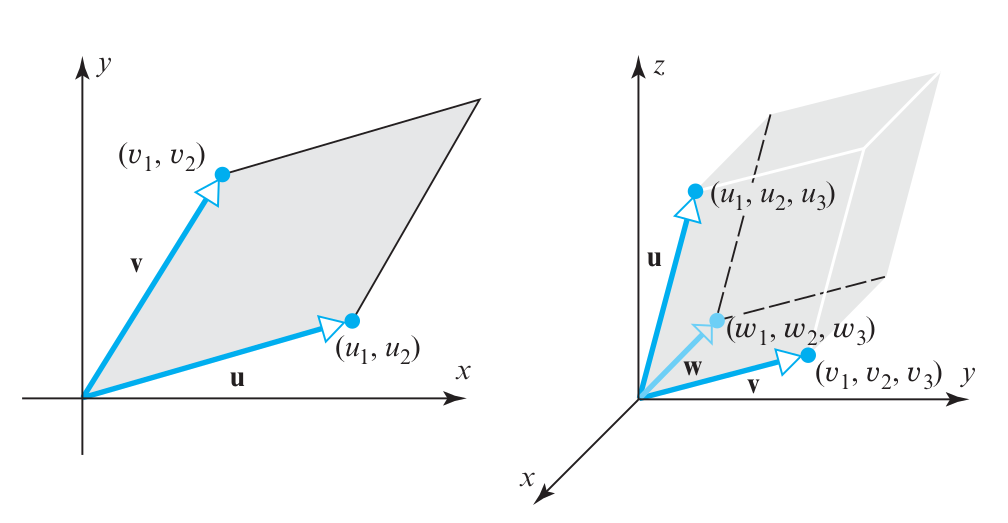
\includegraphics[scale=0.3]{figures/determ.png}
\end{center}
\subsubsection{Calcolo del determinante}
Il determinante di una matrice è una funzione $det: \mathbb{R}^{nn} \Longrightarrow \mathbb{R}$ che verifica queste due proprietà:
\begin{enumerate}
    \item Se $a $ è un numero reale, ossia una matrice di ordine uno quadrata, allora $det(a) = a$ .
    \item   Se A = $\begin{bmatrix}a_{11} & a_{12}a_{21} & a_{22}\end{bmatrix}$ allora $det(A) = a_{11}a_{22} - a_{12}a_{21}$
\end{enumerate}
Dallo sviluppo del caso due notiamo che compaiono due addendi ciascuno dei quali è il prodotto di due fattori. I due fattori nei due prodotti di iniziano entrambi uno con un $1$ e uno con un $2$ per poi seguire con le \textit{permutazioni di $(1,2): (1,2),(2,1)$.} Perché il secondo prodotto ha un $-$ davanti? Il segno è dettato dalla \textit{parità} della permutazione, ovvero: per arrivare alla coppia $(1,2)$ si devono attuare degli scambi, se il numero di scambi è pari, il segno non cambia, se gli scambi sono dispari, il segno cambia.


\begin{es}{esempio}
\begin{align*}
A=
\begin{bmatrix}
a_{11} & a_{12} & a_{13} \\ 
a_{21} & a_{22} & a_{23}  \\
a_{31} &a_{32} & a_{33} 
\end{bmatrix} \rightarrow
det(A) &= a_{11} a_{22} a_{33} + a_{13} a_{21} a_{32} \textcolor{Brown2}{-} a_{11} a_{23} a_{32} \textcolor{Brown2}{-} a_{13} a_{22} a_{31} \textcolor{Brown2}{-} a_{12} a_{21} a_{33} \\
&= \sum_{\sigma} \epsilon (\sigma)a_{1\sigma(1)}a_{2\sigma (2)}a_{3\sigma(3)}
\end{align*}
\end{es}

\begin{center}
\fboxsep11pt
\colorbox{myblue}{\begin{minipage}{5.75in}
\begin{blues}{Definizione: determinante}
Il determinante di una matrice quadrata $A = (a_{ij})$ di ordine $n$ è dato da: 
$$
\sum_{\sigma} \epsilon (\sigma)a_{1\sigma(1)}a_{2\sigma (2)}\dots a_{n\sigma(n)}
$$
dove $\sigma$ è una qualsiasi permutazione dei numeri $1,2,\dots,n$ e $\epsilon(\sigma)$ è il suo segno. 
\end{blues}
\end{minipage}}        
\end{center}

\subsubsection{Come cambia il determinante dopo le 3 mosse?}
\begin{enumerate}
    \item $det^t(A) = det(A)$;
    \item Se $A'$ si ottiene scambiando due righe o due colonne di $A$, allora $det(A') = -det(A)$;
    \item Se faccio moltiplico una riga per un numero reale $\lambda$ allora $det(A^1) = \lambda^n det(A)$;
    \item Se addiziono a una riga un multiplo di un'altra riga il determinante non cambia;
    \item Una matrice con due righe o colonne uguali ha determinante nullo;
    \begin{enumerate}
        \item data la matrice $A \in \mathbb{R}^{n,n}$, $rk(A) = n \longleftrightarrow det(A) \neq 0$
        \item analogamente $rk(A) < n \longleftrightarrow det(A) = 0$
    \end{enumerate}
            
    \item $det(A+B) \neq det(A) + det(B)\quad \forall A,B \in \mathbb{R}^{n,n}$
\item \colorbox{myred}{\begin{minipage}{3.5in}\textbf{Teorema di Binet}: $det(AB) = det(A) det(B) \quad \forall A,B \in \mathbb{R}^{n,n}$;\end{minipage}}
    \item $det(A^{-1}) = (det(A))^{-1}$;
\end{enumerate}

\begin{es}{dimostrazione determinante (2)}
È conseguenza della definizione di determinante e del fatto che lo scambio di due righe comporta il cambiamento di segno di ciascuna permutazione. Per esempio, nel caso della matrice quadrata di ordine 2 si ha:    

$$
\begin{vmatrix}
    a_{11} & a_{12} \\
    a_{21} & a_{22}
\end{vmatrix}
= a_{11}a_{22} - a_{12}a_{21}
$$
Se scambio due righe:
$$
\begin{vmatrix}
    a_{21} & a_{22} \\
    a_{11} & a_{12} 
\end{vmatrix}
= - a_{22}a_{11} + a_{21}a_{12}
$$
\QEDA
\end{es}
\begin{es}{dimostrazione determinante (5a)}
    Operando su una matrice $A$ e la rendo $A'$ a scala triangolare superiore. So allora che $det(A')=\lambda \cdot det(A)$ e $det(A) \neq 0 \Leftrightarrow det(A') \neq 0$.
    Quindi $a'_{ij} \neq 0 \quad \forall j \in \{1,\dots,n\}$.

    Cioè $A'$ ha $n$ righe non nulle, quindi $rk(A') = n$.
\QEDA
\end{es}
\begin{es}{dimostrazione determinante (8)} 
Per il teorema di Binet:
$$
AA^{-1} = I \qquad A^{-1} = \frac{I}{A} \qquad det(A^{-1}) = det(\frac{I}{A}) = \frac{1}{det(A)}
$$
\QEDA
\end{es}





\vspace{1em}
\noindent
\paragraph{osservazioni su matrici inverse}
Se il determinante di una matrice è uguale a zero, significa che la matrice è non invertibile. Questo perché il determinante descrive, anche se non esplicitamente, il numero di soluzioni del sistema di equazioni associato.

\noindent
Il determinante è infatti strettamente legato al \textbf{rango}: se il rango, ovvero il numero di righe non nulle, di una matrice $A \in \mathbb{R}^{r,n}$ è minore di $n$ sappiamo che il determinante vale $0$ e che di conseguenza il sistema\textit{ non può avere una singola soluzione}. Infatti se la matrice ha una riga nulla o più, le soluzioni saranno infinite e legate a uno o più parametri liberi.

\noindent
Se il sistema associato alla matrice $A$ non ha una singola soluzione è chiaro come non possa esistere una matrice $A'$ inversa che soddisfi:
$$
AA^{-1}= I \quad A^{-1} = \frac{I}{A}
$$
L'equazione ha infatti una sola soluzione se e solo se $A$ fosse unicamente definita.

% \subsection{Equazioni matriciali}
% Per equazioni matriciali si intende un'equazione le cui incognite sono matrici del tipo:
% $$
% AX = B
% $$
% $$
% \begin{pmatrix}a_{11}&a_{12}&\cdots &a_{1n}a_{21}&a_{22}&\cdots &a_{2n}\vdots &\vdots &\ddots &\vdots a_{r1}&a_{r2}&\cdots &a_{rn}\end{pmatrix}
% \begin{pmatrix}x_{11}&x_{12}&\cdots &x_{1n}x_{21}&x_{22}&\cdots &x_{2n}\vdots &\vdots &\ddots &\vdots x_{r1}&x_{r2}&\cdots &x_{rn}\end{pmatrix} = 
% \begin{pmatrix}b_{11}&b_{12}&\cdots &b_{1n}b_{21}&b_{22}&\cdots &b_{2n}\vdots &\vdots &\ddots &\vdots b_{r1}&b_{r2}&\cdots &b_{rn}\end{pmatrix}
% $$
% con $A \in \mathbb{R}^{r,n}$, $X \in \mathbb{R}^{n,p}$, $B \in \mathbb{R}^{r,p}$.
% La risoluzione si riconduce a quella di un sitema lineare del tipo:
% $$
% {\begin{cases}a_{11}x_{11}+a_{12}x_{21}+\cdots +a_{1n}x_{n1}=b_{11}a_{11}x_{12}+a_{22}x_{22}+\cdots +a_{2n}x_{n}=b_{2}\vdots a_{11}x_{1p}+a_{12}x_{2p}+\cdots +a_{1n}x_{np}=b_{1p}\end{cases}}
% $$

\subsection{Teoremi di Laplace}
I teoremi di Laplace permettono di semplificare i conti nel calcolo del determinante di una matrice $n \times n$  a conti di un determinante $(n-1) \times (n-1)$. I conti vengono semplificati perché si procede a scegliere un elemento $a_{ij}$ nella matrice (vedremo perché di solito è uno in una riga o colonna con tanti zeri) , "nascondendo" tutti gli elementi della riga e colonna del nostro candidato e andremo a calcolare il determinante della matrice "rimanente", questo determinante lo chiameremo \textbf{minore} di $a_{ij}$  e lo indichiamo con $M_{ij}$.
Ora serve definire il \textbf{cofattore}; il cofattore di $a_{ij}$ è il numero $A_{ij}$ definito dalla formula:
$$
A_{ij}  = (-1)^{ij}\cdot M_{ij}
$$
Vediamo come il fattore $(-1)^{ij}$ da segno positivo o negativo se la posizione di $a_{ij}$ è pari o dispari ($a_{11}$ è pari, $a_{12}$ è dispari...). 

\subsubsection{Primo Teorema di Laplace}
Fissata la riga i-esima, il determinante di una matrice quadrata $A \in \mathbb{R}^{n,n}$ è dato dalla somma di tutti i prodotti tra gli elementi della riga e i rispettivi cofattori (questo metodo funziona anche con le colonne) :
$$
\text{det}(A) = \sum_{j=1}^{n}a_{ij}A_{ij}
$$
\subsubsection{Secondo Teorema di Laplace}
In una matrice quadrata $A \in \mathbb{R}^{n,n}$ la somma dei prodotti tra gli elementi di una riga (o colonna) e i  cofattori \textit{di una riga parallela} è zero:
\begin{align*}
  0 &= \sum_{k=1}^{n}a_{ik}A_{jk}  \\
    &= \sum_{h=1}^{n}a_{hi}A_{hj} \qquad i \neq j
\end{align*}



\begin{es}{verifica}
    % Abbiamo visto nel primo teorema che ciascuno dei cofattori  $A_{ij}$ "\textit{non vede}" la riga i-esima, quindi:
    È conseguenza evidente della proprietà $(2)$ del determinante secondo la quale \textit{se scambio due righe o colonne a una matrice allora il suo determinante cambia di segno.} Si puó interpretare come lo sviluppo del determinante di un matrice in cui, nel primo caso, la riga j-esima coincide con la riga i-esima e nel secondo caso, la colonna j-esima coincide con la riga i-esima.
    $$
    A = \begin{bmatrix}
        a & b & c \\
        d & e & f \\
        g & h & i
    \end{bmatrix} 
    $$
    Se per esempio scegliamo di moltiplicare gli elementi della prima riga per i complementi della seconda abbiamo:
    $$
    a\begin{vmatrix}
        b & c \\
        h & i
    \end{vmatrix}
    -b\begin{vmatrix}
        a & c \\
        g & i
    \end{vmatrix}
    +c\begin{vmatrix}
        a & b \\
        g & h
    \end{vmatrix}
    $$
    $$
    = abi - ach - bai + bcg + cah - cbg = 0
    $$
\end{es}


%MATRICI INVERSE
\subsection{Matrici inverse}
\begin{center}
\fboxsep11pt
\colorbox{myblue}{\begin{minipage}{5.75in}
\begin{blues}{Definizione: matrice invertibile}
    Una matrice $A \in \mathbb{R}^{n,n}$ si dice invertibile se $\exists$ una matrice $X$ tale che $AX = XA = I$.
\end{blues}
\end{minipage}}        
\end{center}
\subsubsection*{Proprietà generali delle matrici inverse}
\begin{enumerate}
    \item Se esiste una matrice inversa allora questa è univocamente determinata e la chiamo $A^{-1}$;
    \item $(AB)^{-1} = B^{-1}A^{-1}$;
    \item Se $A,B$ sono invertibili non è detto che lo sia $A+B$;
    \item $(\leftindex ^t{A})^{-1} = \leftindex ^t(A^{-1})$.
\end{enumerate}



\begin{es}{dimostrazione (1)}
Supponiamo che $X$ e $X'$ soddisfino:
$$
XA = I = AX 
$$
$$
X' A = I = AX'
$$
$$
XAX = \begin{array}{c}
       (XA)X' = IX' = X' \\
       X(AX') = XI = X
    \end{array}
    \rightarrow
    XA = AX'
$$
Abbiamo dimostrato che se esiste una $X$ inversa a sinistra per $A$ ed esiste una $X' $ inversa a esa per $A$, allora $X=X'$ e quindi $A$ è invertibile e X è la sua inversa.
\end{es}
\begin{es}{dimostrazione (2)}
Vedo se la candidata ad inversa $B^{-1}A^{-1}$ soddisfa le proprietà richieste:
$$
(B^{-1}A^{-1})AB = B^{-1}(A^{-1}A)B = B^{-1}IB = B^{-1}B = I
$$
$$
AB(B^{-1}A^{-1})= \dots = I
$$
\QEDA
\end{es}

\begin{center}
\fboxsep11pt
\colorbox{myred}{
\begin{minipage}{5.75in}
\begin{redes}{Teorema}
Sia A una matrice quadrata di ordine $n$, se $\text{det}(A) \neq 0$ allora esiste l’inversa di $A$ ed è:
\[
A^{-1} = \frac{1}{\text{det}(A)}\text{adj}(A)
\]
\end{redes}
\end{minipage}}
\end{center}

\begin{es}{dimostrazione}
Dai teoremi di Laplace so che:
\[
	\sum_{j=1}^n a_{ij}A_{kj} = \left\{\begin{array}{c} \text{det}A \quad \text{se} \quad i = k \\ 0 \quad \text{se}\quad i \neq k \end{array} \right
.\] 
ovvero che la somma dei prodotti tra tutti gli elementi di una riga di $A$ e i rispettivi cofattori è uguale o a $0$ o al determinante di A.

Ovvero che il prodotto tra la matrice $A$ e la trasposta della matrice dei cofattori di A ($\text{adj}A$) si può scrivere come:
\[
A \cdot \text{adj}A = \begin{bmatrix}
	\text{det}A & 0 & \dots & 0 \\
	0 & \text{det}A & \dots & 0\\
	\vdots & 0 &  \ddots & 0 \\

\end{bmatrix}
= \text{det}A \cdot I
\]
Possiamo notare quindi che dopo le opportune operazioni ci si riconduce alla formula iniziale.
\QEDA
\end{es}


\begin{center}
\fboxsep11pt
\colorbox{myred}{\begin{minipage}{5.75in}
\begin{redes}{Teorema}
Una matrice $A$ è invertibile  $\Longleftrightarrow$ il rango è massimo ($\text{rk}A = n$).

Possiamo dire che risolvere $Ax = I$ sia equivalente a scrivere  $x$ per colonne e risolvere il seguente sistema:
\[
	\left(*\right) \left\{ \begin{array}{c} A\overline{x}_{1} = \left(1,0,\dots,0\right) \\ A\overline{x}_{2} = \left(0,1,\dots,0\right) \\ \vdots\end{array}\right
.\] 
\end{redes}
\end{minipage}}        
\end{center}

\begin{es}{dimostrazione}
$\Rightarrow \text{(dimostro che il rango è massimo)}\quad $ So che $A$ è invertibile: esiste  $A^{-1}$.

Considero:
$$
\textcolor{red}{A^{-1}} A \cdot \overline{x}_{1} = \textcolor{red}{A^{-1}}
\begin{bmatrix}
1\\ 0 \\ \vdots \\ 0 
\end{bmatrix} \quad \Rightarrow \quad 
I \cdot \overline{x}_{1} = A^{-1}
\begin{bmatrix}
 1\\ 0 \\ \vdots \\ 0 
\end{bmatrix} 
\quad \Rightarrow \quad 
\overline{x}_{1} = A^{-1}
\begin{bmatrix}
 1\\ 0 \\ \vdots \\ 0 
\end{bmatrix} 
$$
\[
\Rightarrow \quad \text{esiste una sola soluzione} \quad \Rightarrow \quad \text{par. lib.} = 0 \quad \Rightarrow \quad \text{rk}A = n
\] 	 


\end{es}



\subsubsection{Calcolo della matrice inversa 1}
Il primo metodo consiste nello svolgimento di un'equazione matriciale:
$$
AX = I
$$
Che si risolve come:
$$
(A|I) = \left[\begin{array}{cccc|cccc}
    a_{11} & a_{12} & \dots & a_{1n} & 1 & 0& \dots & 0 \\
    a_{21} & a_{22} & \dots & a_{2n} & 0 & 1& \dots & 0 \\
    \vdots & \vdots & \ddots & \vdots &  \vdots &  \vdots& \ddots & \vdots \\
    a_{n1} & a_{n2} & \dots & a_{nn} & 0 & 0& \dots & 1 \\
\end{array}\right]
$$

\subsubsection{Calcolo della matrice inversa 2}
Possiamo calcolare la matrice inversa anche a partire dalla nozione di determinante dopo aver parlato dei teoremi di Laplace.

\begin{center}
\fboxsep11pt
\colorbox{myblue}{\begin{minipage}{5.75in}
\begin{blues}{Definizione: matrice aggiunta}
Si dice \textbf{matrice aggiunta} di $A$ la trasposta della matrice contentente i \textit{cofattori } di $A$:
$$
\text{Adj}(A)_{ij} = [A_{ij}]
$$
Per esempio:
$$
A=\begin{bmatrix}
    1 &2&3 \\
-1&2&5 \\
0 &1&2
\end{bmatrix}
\qquad
\text{Adj}(A) = \begin{bmatrix}
    -1 &-1 &4 \\
2 &2 &-8 \\
-1 &-1& 4
\end{bmatrix}
$$
\end{blues}
\end{minipage}}        
\end{center}

I teoremi di Laplace più la matrice adiacente ci permettono di  determinare in modo esplicito la formula dell'inversa.


%CRAMER
\subsection{Teorema di Cramer}
Subito dopo aver descritto un nuovo modo per calcolare la matrice inversa vediamo come può tornare utile nella risoluzione di sistemi lineari con $n$ incognite e $n$ equazioni.
$$
A\overline{x} = \overline{b}
$$
$$
\overline{x} = A^{-1}\overline{b}
$$
$$
\overline{x} = \frac{1}{\text{det}(A)}\text{adj}(A) \cdot \overline{b}
$$
$$
\overline{x} = \begin{bmatrix}
    x_1 \\ x_2 \\ \vdots\\  x_n
\end{bmatrix} = \frac{1}{\text{det}(A)}
\begin{bmatrix}
    A_{11} & A_{12} & \dots & A_{1n} \\
    A_{21} & A_{22} & \dots & A_{2n}  \\
    \vdots & \vdots & \ddots & \vdots  \\
    A_{n1} & A_{n2} & \dots & A_{nn}
\end{bmatrix}
\begin{bmatrix}
    b_1 \\ b_2 \\ \vdots\\  b_n
\end{bmatrix}
= \frac{1}{\text{det}(A)}
\begin{bmatrix} 
    A_{11}b_1 & A_{12}b_2 & \dots & A_{1n}b_n  \\
    A_{21}b_1 & A_{22}b_2 & \dots & A_{2n}b_n  \\
    \vdots & \vdots & \ddots & \vdots \\
    A_{n1}b_1 & A_{n2}b_2 & \dots & A_{nn}b_n 
\end{bmatrix}
$$

da cui: 
\begin{align*}
    x_i &= \frac{1}{\text{det}(A)}(b_1 A_{2i} + b_2  A_{2i} + \dots + b_nA{ni})  \\
   &= \frac{1}{\text{det}(A)} \text{det}(\overline{a}_1 | \overline{a}_2 \dots |\overline{b}| \dots |\overline{a}_n)
\end{align*}



%% %% %%
%% %% %%  PRODOTTO SCALARE e VETTORIALE
%% %% %% 

\newpage
\section{Prodotto scalare e vettoriale}
Prima di parlare di prodotto scalare è necessario introdurre due concetti fondamentali:

\begin{enumerate}
	\item \textbf{Lunghezza} di un vettore che d'ora in poi chiameremo \textit{norma};
	\item \textbf{Angolo} tra due vettori.
\end{enumerate}

\begin{center}
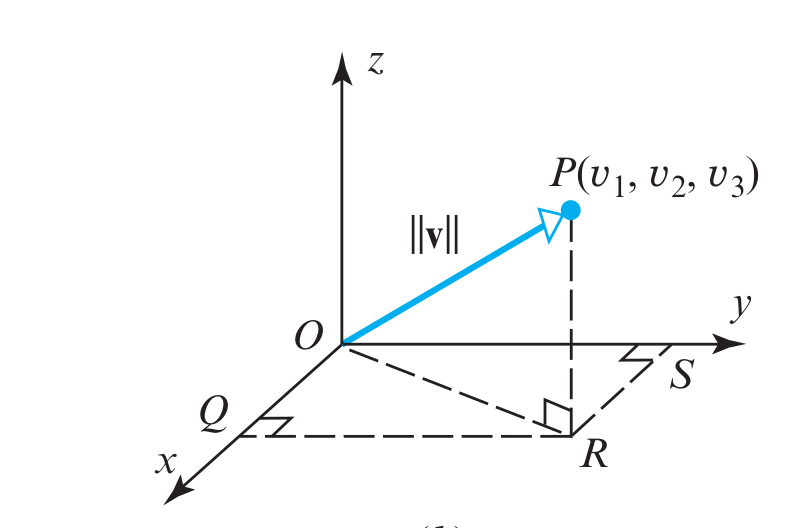
\includegraphics[scale=0.2]{figures/norma.png}
\end{center}

La norma del vettore è definita dalla formula:
\[
\|v\| = \sqrt{v_1^2 + v_2^2 + \dots + v_{n}^2}
.\] 

Vedremo come saranno di estrema importanza i vettori di norma 1, o vettori unitari. Per esempio in $V_3$ i vettori unitari sono $i,j,k$. In generale per \textit{normalizzare} un vettore basta dividerlo per la sua lunghezza, quindi per la sua norma:
\[
u = \frac{v}{\|v\|}
.\] 


\begin{center}
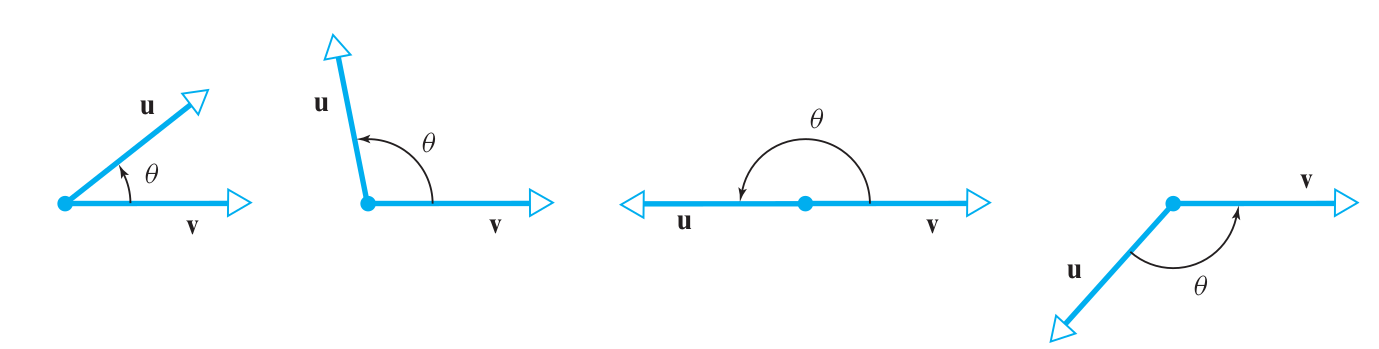
\includegraphics[scale=0.25]{figures/angoli.png}
\end{center}
Per quanto riguarda l'angolo tra due vettori invece prenderemo in considerazione solo la parte compresa tra $0$ e $\pi$.


Ora che sappiamo cosa sono norma di un vettore e angolo tra vettori possiamo parlare di \textbf{prodotto scalare}. E' infatti necessario introdurre un'operazione moltiplicativa "utile" per vettori in $\mathbb{R}^2$ e in $\mathbb{R}^3$.

\begin{center}
\fboxsep11pt
\colorbox{myblue}{\begin{minipage}{5.75in}
\begin{blues}{Definizione: prodotto scalare}
Il prodotto scalare (in $V_3$ ) $x\cdot y$ di due vettori $x$ e $y$ in $V_3$ è la funzione:
\[
\cdot : \quad V_3 \times V_3 \quad \longrightarrow \quad \mathbb{R}
.\] 
così definita:
\[
x \cdot y  = \|x\| \|y\| \cos{\hat{xy}}
.\] 

\end{blues}
\end{minipage}}        
\end{center}

Dalla definizione troviamo altre due espressioni di norma e angolo (notare come ora il concetto di angolo sia esteso a tutto $\mathbb{R}^n$):
\[
\|v\| = \sqrt{v\cdot v} \qquad \qquad \cos{\theta} = \frac{u\cdot v}{\|u\|\|v\|}
.\]

\subsection{Proprietà del prodotto scalare}
\begin{itemize}
	\item $x \cdot y$ = $y \cdot x \quad \forall x,y \in V_3$;
	\item $\left(x + y\right)\cdot z = x\cdot z + y\cdot z$;
	\item $\left(\lambda x\right)\cdot z = \lambda x \cdot z = x \cdot \left(\lambda z\right)$;
	\item $x\cdot x \geq 0 \qquad = 0 \Longleftrightarrow x = 0$.
\end{itemize}

\subsection{Interpretazione geometrica del prodotto scalare}
Il prodotto scalare $\|a\|\|u\|\cos{\theta}$ non è altro che il prodotto della lunghezza di uno dei due vettori ($\|a\|$) per la proiezione ortogonale con segno dell'altro sul primo($\|u\|\cos{\theta}$).

\begin{center}
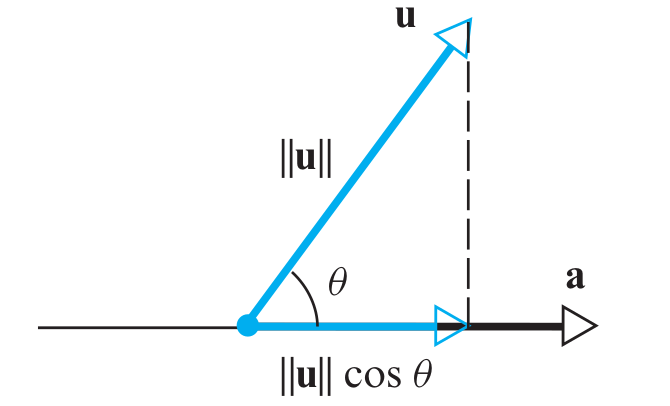
\includegraphics[scale=0.25]{figures/proj.png}
\end{center}


\begin{center}
\fboxsep11pt
\colorbox{myred}{\begin{minipage}{5.75in}
\begin{redes}{Teorema: vettore proiezione ortogonale}
Dati due vettori $x$ e $y$ non nulli il vettore proiezione ortogonale di $y$ su $x$ è:
\[
p = \frac{x\cdot y}{\|x\|^2}x
.\] 
\end{redes}
\end{minipage}}        
\end{center}

\begin{es}{dimostrazione}
Il mio obiettivo è quello di scrivere la proiezione di $u$ su $a$ in questa forma:
\[
p = * \frac{a}{\|a\|}
.\] 
dove "*" indica la lunghezza della proiezione.
Guardando la figura in alto sappiamo che la proiezione $\|p\| = \|u\|\cos{\theta}$. Quindi:
\[
p = \|u\|\cos{\theta} \frac{a}{\|a\|} 
.\] 
Per elimiare il coseno di theta risaliamo alla formula di prodotto scalare:
\[
u \cdot a = \|u\|\|a\|\cos{\theta} \quad \longrightarrow \quad \|u\|\cos{\theta} = \frac{u\cdot a}{\|a\|}
.\] 
Quindi:
\[
p = \frac{u\cdot a}{\|a\|^2}a
.\] 
\end{es}


\begin{center}
\fboxsep11pt
\colorbox{myred}{\begin{minipage}{5.75in}
\begin{redes}{Teorema di Pitagora generalizzato}
Dati $u$ e $v$ vettori ortogonali tra loro in $\mathbb{R}^n$ con prodotto standard, allora
\[
\|u+v\|^2 = \|u\|^2 + \|v\|^2
.\] 
\textit{la dimostrazione è molto semplice, il termine $2u\cdot v$ vale zero.}
\end{redes}
\end{minipage}}        
\end{center}


\subsection{Prodotto vettoriale}

\begin{center}
\fboxsep11pt
\colorbox{myblue}{\begin{minipage}{5.75in}
\begin{blues}{Definizione: prodotto vettoriale}
Il prodotto vettoriale (in $V_3$ ) $x\cdot y$ di due vettori $x$ e $y$ in $V_3$ è la funzione:
\[
\wedge : \quad V_3 \times V_3, \quad \longrightarrow \quad \left(x,y\right) \mapsto x \wedge y
.\] 
così definita:
\[
x \wedge y  = \|x\wedge y\| \|x\| \|y\| \sin{\hat{xy}}
.\] 

\end{blues}
\end{minipage}}        
\end{center}
Il verso del vettore risultante dal prodotto vettoriale ha il verso che segue la \textit{regola della mano destra}.


\noindent
Possiamo anche scrivere il prodotto scalare tramite lo sviluppo di determinanti in questo modo:
\[
u \wedge v = 
\begin{vmatrix}
     i& j & k \\
     u_1& u_2 & u_3 \\
     v_1& v_2 & v_3 
\end{vmatrix}
\] 

\[
	=
\left(
\begin{vmatrix}
    u_2 & u_3  \\
     v_2& v_3  
\end{vmatrix}i,
- \begin{vmatrix}
    u_1 &u_3 \\
     v_1&v_3   
\end{vmatrix}j, +
\begin{vmatrix}
    u_1 & u_2 \\
     v_1 &  v_2   
\end{vmatrix}k
\right)
.\] 

\subsubsection{Proprietà del prodotto vettoriale}
\begin{itemize}
	\item $u \wedge v = -\left(v\wedge u\right)$ ;
	\item $u \wedge \left(v+w\right) = u\wedge v + u \wedge w$;
	\item $k\left(u\wedge v\right) = ku \wedge v = u \wedge kv$ ;
	\item $u \wedge u = 0$
\end{itemize}

\subsubsection{Interpretazione geometrica del prodotto vettoriale}
Dati $u$ e $v$ vettori in uno spazio tridimensionale, dall'identità di Lagrange sappaiamo che:
\begin{align*}
	\|u\wedge v\|^2 &= \|u\|^2\|v\|^2 - \left(u\cdot v\right)^2 \\
			&= - \|u\|^2\|v\|^2\cos{\theta}^2 \\
			&= \|u\|^2\|v\|^2 \left(1-\cos{\theta}^2\right) \\
			&= \|u\|^2\|v\|^2 \sin{\theta}^2 \\
\end{align*}
\noindent
Da questo possiamo notare che il prodotto vettoriale può essere inteso anche come area del parallelogramma che ha come lati i due vettori. 

\begin{center}
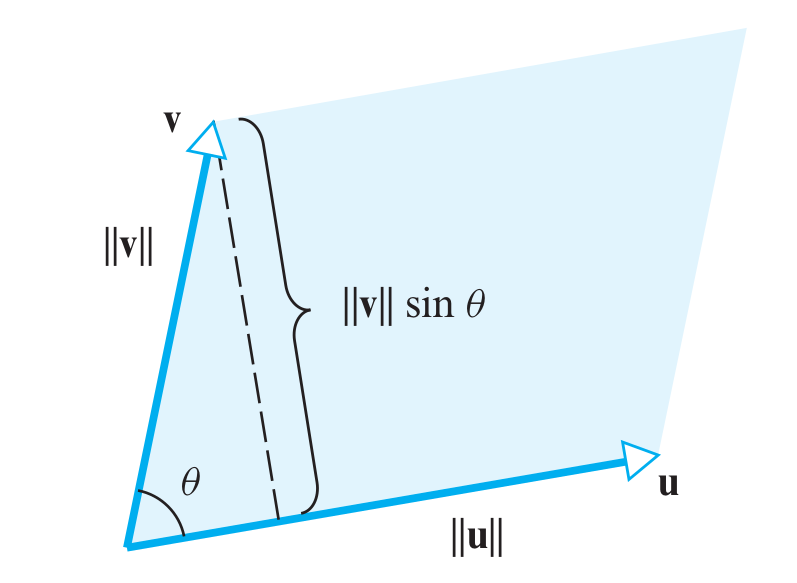
\includegraphics[scale=0.25]{figures/uedge.png}
\end{center}

\subsection{Prodotto misto}

\begin{center}
\fboxsep11pt
\colorbox{myblue}{\begin{minipage}{5.75in}
\begin{blues}{Definizione: Prodotto misto}
Dati due vettori $u$ e $v$, allora
\[
u \cdot \left(v \wedge w\right)
.\] 
è chiamato prodotto misto di $u$ $v$ e  $w$.
\end{blues}
\end{minipage}}        
\end{center}
Geometricamente il prodotto misto rappresenta $\frac{1}{6}$ del volume del tetraedro formato dai tre vettori.


%% %% %%
%% %% %%  SPAZI VETTORIALI
%% %% %% 

\newpage
\section{Spazi Vettoriali}
\begin{center}
\fboxsep11pt
\colorbox{myblue}{\begin{minipage}{5.75in}
\begin{blues}{Definizione: Spazio Vettoriale}
    Si definisce \textbf{spazio vettoriale} sul campo dei numeri reali $\mathbb{R}$ un certo insieme $V$ nel quale sono definite le seguenti operazioni:
    \begin{enumerate}
        \item somma $+$: $V \times V \longrightarrow V$.
        \item prodotto $\cdot$: $\mathbb{R} \times V \longrightarrow V$.
        \end{enumerate}
	Un gruppo $\left(V,\times \right)$ si dice \textit{commutativo} (o Abeliano) se $v \times y = y \times x \quad \forall x,y \in V$
\end{blues}
\end{minipage}}        
\end{center}


\subsubsection{Proprietà della somma}
\begin{enumerate}
    \item commutativa: $x + y = y + x, \quad \forall x,y \in V$
    \item associativa: $(x+y)+z = x + (y+z),\quad \forall x,y \in V$
    \item esistenza dell'elemento neutro: $\exists 0 \in V : 0 + x = x +0, \quad \forall x,y \in V$
    \item esistenza dell'opposto: $\forall x \in V \exists -x \in V : x + (-x) = (-x) +x = 0$
\end{enumerate}
\subsubsection{Proprietà del prodotto}
\begin{enumerate}
    \item (diciamo) distributiva: $\lambda(x+y) = \lambda x + \lambda y,\quad \forall x,y \in V, \forall \lambda \in \mathbb{R}$
    \item $(\lambda + \mu)\cdot \overline{x} = \lambda \overline{x} + \mu \overline{x}, \quad \forall x,y \in V, \forall \lambda \in \mathbb{R}$
    \item $(\lambda \cdot \mu)\overline{x} = \lambda(\mu \cdot \overline{x}),\quad \forall x,y \in V$
    \item $1 \cdot \overline{x} = \overline{x}, \quad \forall x,y \in V$
\end{enumerate}



\subsection{Sottospazi vettoriali}
\begin{center}
\fboxsep11pt
\colorbox{myblue}{\begin{minipage}{5.75in}
\begin{blues}{Definizione: sottospazio vettoriale}
Sia $V$ uno spazio vettoriale reale, $W \subseteq V $ è un sottospazio vettoriale di $V$ se $W$ è uno spazio vettoriale rispetto alle stesse operazioni di $V$, quindi rispetto alle operazioni di \textit{somma} e \textit{prodotto}.

\begin{itemize}
	\item Se ho 2 elementi $\overline{x},\overline{y}\in W \quad \Rightarrow \quad \overline{x} + \overline{y} \in W$;
	\item Se ho 2 elementi $\overline{x} \in W, \lambda \in \mathbb{R} \quad \Rightarrow \quad \lambda\overline{x} \in W$.
\end{itemize}

\end{blues}
\end{minipage}}        
\end{center}

\begin{center}
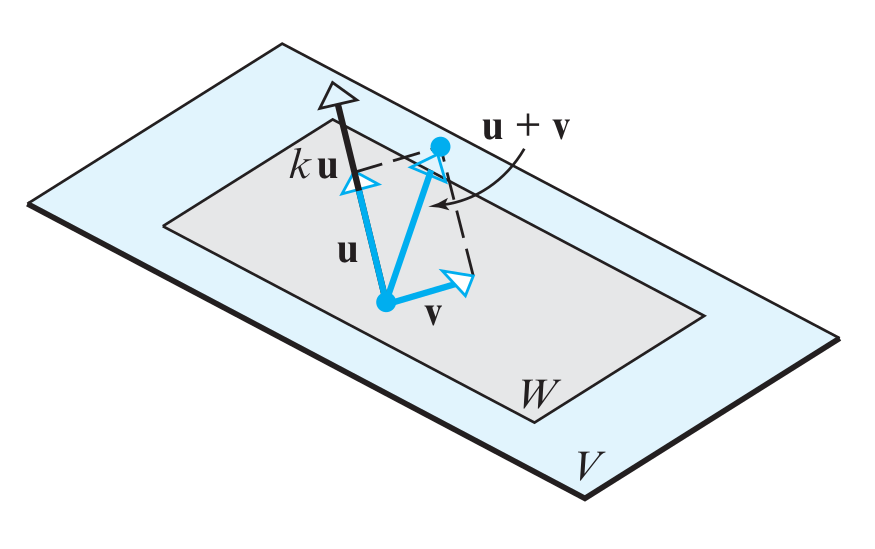
\includegraphics[scale=0.25]{figures/subspace.png}
\end{center}
In figura vediamo come $u$ e $v$ siano contenuti in $W$ ma la loro somma no.

\begin{es}{Esempio fondamentale di sottospazio vettoriale}
L'insieme delle soluzioni di un sistema lineare omogeneo di $m$ equazioni in $n$ incognite è un sottospazio vettoriale di $\mathbb{R}^n$. L'insieme delle soluzioni di 
\[
AX = O \qquad A \in \mathbb{R}^{m,n}, X \in \mathbb{R}^{n,1}, O \in \mathbb{R}^{m,1}
\] 
è detto \textit{nullspace} e coincide con l'insieme

\[
N\left(A\right) = \left\{ X \in \mathbb{R}^n | AX = O  \right\}
\]

Dati $X_1$ e $X_2$ $\in N\left(A\right)$ si deve dimostrare che 
\[
\lambda X_1 è \mu X_2 \in N\left(A\right) \quad \forall \lambda,\mu \in \mathbb{R}
\] 
che sviluppando
\[
A\left(\lambda X_1 + \mu X_2\right) = \lambda AX_1 + \mu AX_2 = O
.\] 
\end{es}


\subsubsection{$+$ Somma di due sottospazi}
La somma di due sottospazi è il più piccolo sottospazio contenente l'unione dei duee si esprime come l'insieme di tutti i vettori ottenuti dalla somma di vettori appartenenti ai sottospazi sommati.
\[
W_1 + W_2  = \left\{\overline{x} \in V: \quad \overline{x} = \overline{y}+\overline{z}  \qquad y \in W_1, \quad z \in W_2\right\}
.\] 

Quindi $W_1 + W_2$ contiene $W_1$ e contiene $W_2$ e $W_1 + W_2$ è sottospazio.
\begin{es}{dimostrazione}
Possiamo dire che è sottospazio se la somma tra ogni vettore ricade in esso così come il prodotto tra ogni vettore e uno scalare.

Prendiamo due vettori $\overline{x}$ e $\overline{y}$ entrambi $\in W_1 + W_2$:
\[
\overline{x} = \overline{x}_{1} + \overline{x}_{2} \quad \overline{x}_1 \in W_1, \quad \overline{x}_{2} \in W_2
.\] 
\[
\overline{y} = \overline{y}_{1} + \overline{y}_{2} \quad \overline{y}_1 \in W_1, \quad \overline{y}_{2} \in W_2
.\] 
\begin{align*}
	\left(+\right)\Rightarrow \quad \overline{x} + \overline{y} &= \overline{x}_{1} + \overline{x}_{2} + \overline{y}_{1} + \overline{y}_{2} \\
						      &= \left(\overline{x}_{1} + \overline{y}_{1}\right) + \left(\overline{x}_{2}+\overline{y}_{2}\right) \quad \Rightarrow \quad \in W_1 + W_2 
\end{align*}
\begin{align*}
	\left(\cdot\right) \Rightarrow \quad \lambda\left(\overline{x}+\overline{y}\right) &= \lambda \overline{x}_{1} + \lambda \overline{x}_{2} + \lambda \overline{y}_{1} + \lambda \overline{y}_{2} \\
						      &= \lambda\left(\overline{x}_{1} + \overline{y}_{1}\right) + \lambda\left(\overline{x}_{2}+\overline{y}_{2}\right) \quad \Rightarrow \quad \in W_1 + W_2
\end{align*}
\end{es}


\begin{center}
\fboxsep11pt
\colorbox{myblue}{\begin{minipage}{5.75in}
\begin{blues}{Definizione: Somma diretta}
$\left(V,+,\cdot\right)$ spazio vettoriale, $W_1,W_2 \leq V$. Diciamo che la somma $W_1+W_2$ è una somma diretta se ogni $\overline{x} \in W_1+W_2$ si scrive in modo unico come $\overline{x}_1 + \overline{x}_2$ con $\overline{x}_1 \in W_1$ e $\overline{x}_2 \in W_2 $.

La somma verrà scritta come:
\[
W_1 \oplus W_2 = V
.\] 
\end{blues}
\end{minipage}}        
\end{center}

\paragraph{Proposizione}
In $V$ spazio vettoriale, $W_1,W_2 \leq V$. Allora:
\[
W_1 \quad \text{e} \quad W_2 \quad \text{sono in somma diretta} \quad \Longleftrightarrow \quad W_1 \cap W_2 = \{\overline{0}\} 
.\] 

\begin{es}{dimostrazione}
\[
\Leftarrow \quad \text{se esiste un x con almeno 2 decomposizioni} \quad \Rightarrow \quad \exists \overline{z} \in W_1 \cap W_2,\quad \overline{z} \neq \overline{0}
.\] 
Prendo allora tale $\overline{x}$ che si scompone in due coordinate x e in due y:
\[
\overline{x}_{1} + \overline{x}_{2} = \overline{x} = \overline{y}_{1} + \overline{y}_{2}, \quad \overline{x}_{1} \neq \overline{x}_{2}, \quad \overline{y}_{1} \neq \overline{y}_{2}
.\] 
\[
\overline{x}_{1} + \overline{x}_{2} = \overline{y}_{1} + \overline{y}_{2}
.\] 
\[
\overline{y}_{1} - \overline{x}_{1} = \overline{x}_{2} - \overline{y}_{2} \quad = \overline{z}
.\] 
Il vettore $\overline{z}$ è contenuto sia in $W_1$ sia in $W_2$, quindi $W_1 \cap W_2 \neq \overline{0}$.

Contronominale: se $W_1 \cap W_2 \neq \{\overline{0}\} \quad \Rightarrow \quad \text{non ho unicità di scrittura}$
\[
\Rightarrow \quad \text{Se} \quad \overline{z} \in W_1 \cap W_2, \quad\overline{z} \neq 0
.\] 
\[
x \in W_1 + W_2
.\] 
\[
\overline{x} = \overline{x}_{1} \textcolor{red}{+\overline{z}} + \overline{x}_{2} \textcolor{red}{-\overline{z}}
.\] 
\QEDA
\end{es}


\subsubsection{$\cap$ Intersezione di due sottospazi}
L'intersezione di due sottospazi vettoriali $W_1$ e $W_2$ contiene tutti i vettori contenuti sia in $W_1$ sia in $W_2$.

\begin{center}
\fboxsep11pt
\colorbox{myred}{\begin{minipage}{5.75in}
\begin{redes}{Teorema: l'intersezione è sottospazio}
Immediata conseguenza delle definizioni di sottospazio vettoriale e di intersezione. Se $W_1$ e $W_2$ sono sottospazi allora lo deve essere anche $W_1 \cap W_2$.
\end{redes}
\end{minipage}}        
\end{center}



\subsection{Combinazione lineare}

\begin{center}
\fboxsep11pt
\colorbox{myblue}{\begin{minipage}{5.75in}
\begin{blues}{Definizione: combinazione lineare}
Dato $V$ spazio vettoriale, $\overline{v}_{1},\dots,\overline{v}_{n} \in V$, una composizione lineare di $\overline{v}_{1},\dots,\overline{v}_{n}$ è una strutura del tipo $\lambda_{1}\overline{v}_{1},\dots,\lambda_{n}\overline{v}_{n}$ con ogni $\lambda \in \mathbb{R}$.
\end{blues}
\end{minipage}}        
\end{center}
Ogni sottospazio possiamo dire essere generato da combinazioni lineari dei vettori che lo generano. 


\begin{center}
\fboxsep11pt
\colorbox{myred}{\begin{minipage}{5.75in}
\begin{redes}{Teorema}
Se $S=\{w_1,w_2,\dots,w_{r}\}$ è un insieme di vettori non nullo contenuto in $V$, allora:  \\
L'insieme  $W = \mathscr{L}\left(\left(w_1\right),\left(w_2\right),\dots,\left(w_{r}\right)\right)$, è il \textbf{più piccolo} sottospazio di V che contiene tutti i vettori di $S$. \\
In questo caso si dice che  $W$  \textbf{è generato} da $S$.
\end{redes}
\end{minipage}}        
\end{center}

\begin{center}
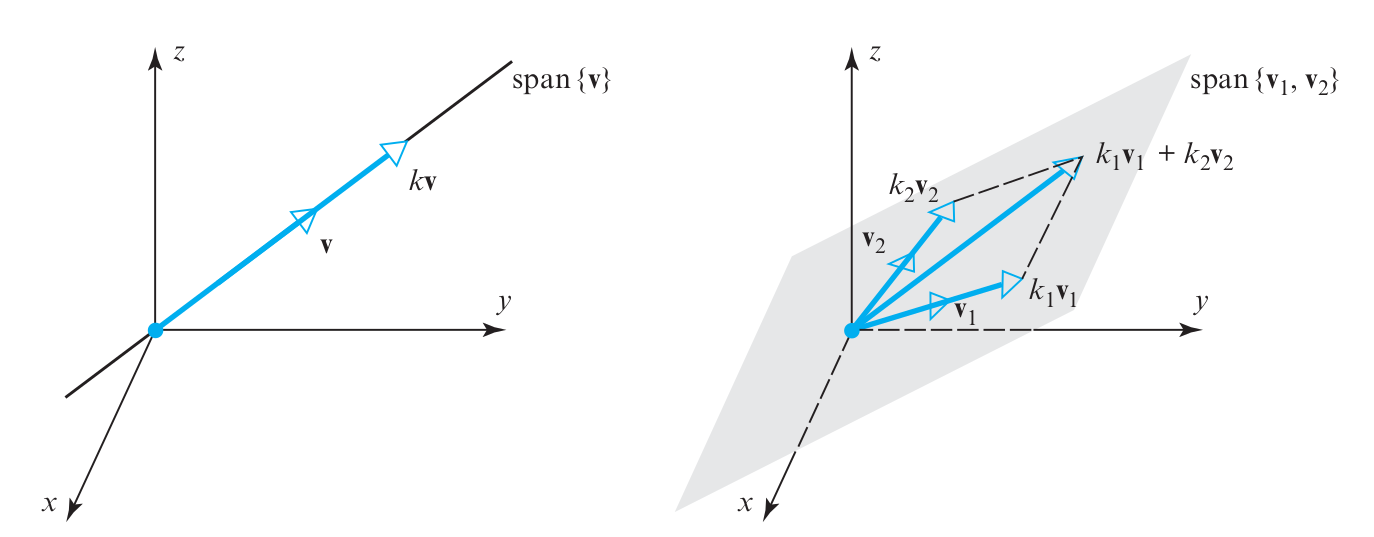
\includegraphics[scale=0.3]{figures/span.png}
\end{center}

\noindent
E' importante riconoscere che gli insiemi di generatori \textit{non sono unici}. Per esempio qualsiasi vettore non nullo sulla linea in figura sarebbe generatore  di $v$. Sono generatori tutte le combinazioni lineari di un insieme di generatori.

\subsection{Indipendenza lineare}
Diciamo di avere uno spazio $xy$ con vettori standard $i$ e $j$. Ogni vettore in $xy$ può essere espresso in modo unico come combinazione lineare di $i$ e $j$. Supponiamo ora di introdurre una terza coordinata $w$ a 45 gradi tra gli assi $x$ e $y$. 

Questo terzo asse risulta essere totalmente superfluo poiché lui stesso può essere espresso come combinazione lineare di $i$ e $j$ per cui non aiuta a descrivere nessun vettore sul piano.


\begin{center}
\fboxsep11pt
\colorbox{myblue}{\begin{minipage}{5.75in}
\begin{blues}{Definizione: Vettori linearmente indipendenti}
Dato un insieme di vettori $V=\{v_1,v_2,\dots,v_{r}\}$, questo  è detto \textit{linearmente indipendente} se nessun vettore in $V$ può essere espresso come combinazione lineare di uno degli altri. Quindi se e solo se:
\[
k_1v_1 + k_2v_2 + \dots + k_rv_r = 0
.\] 
è risolto solo da $k_1 =k_2= \dots = k_r =0$.

Un insieme di vettori linearmente indipendenti si dice \textbf{libero}.
\end{blues}
\end{minipage}}        
\end{center}

\begin{center}
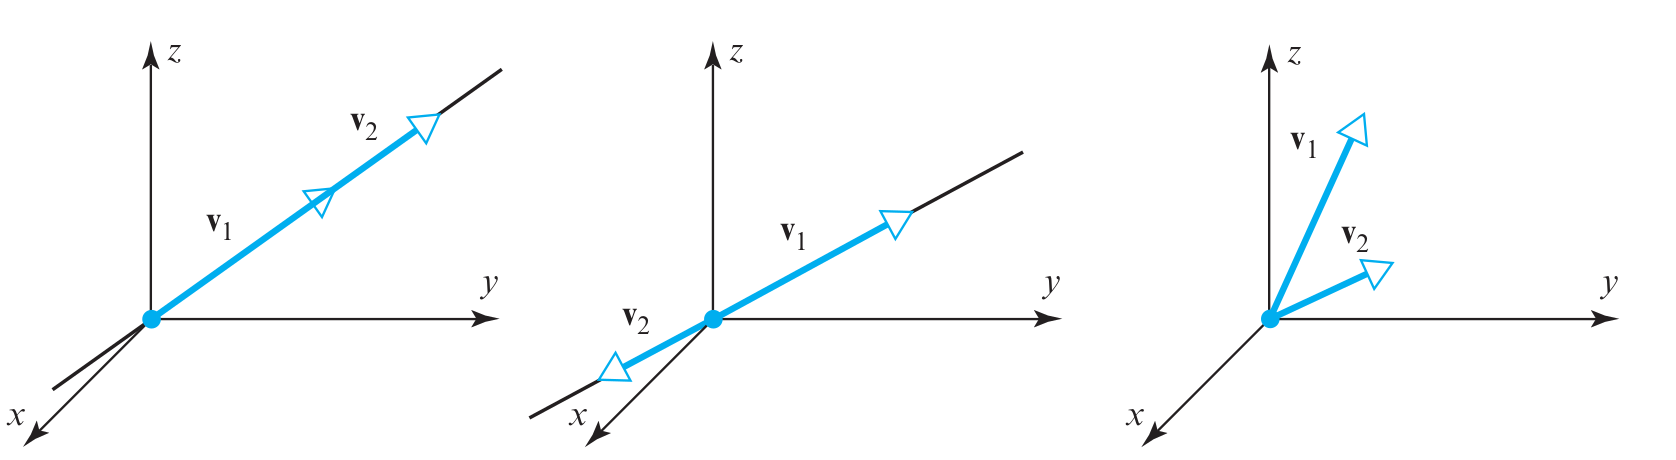
\includegraphics[scale=0.22]{figures/linind.png}
\end{center}
$$
\begin{array}{ccc}
	l.d.\qquad \qquad \qquad \qquad \qquad \qquad& l.i. & \qquad \qquad \qquad \qquad \qquad \qquad l.i. 
\end{array}
$$ 
\begin{center}
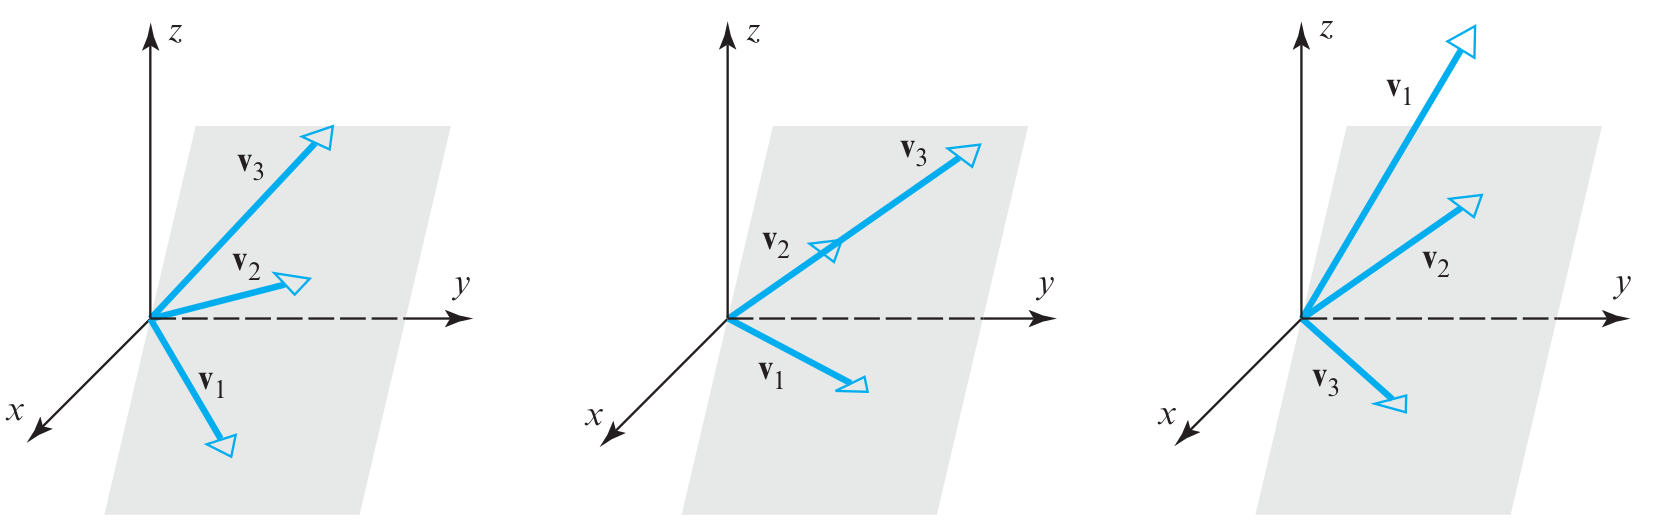
\includegraphics[scale=0.22]{figures/linind2.png}
\end{center}
$$
\begin{array}{ccc}
	l.d.\qquad \qquad \qquad \qquad \qquad \qquad& l.d. & \qquad \qquad \qquad \qquad \qquad \qquad l.i. 
\end{array}
$$

\subsection{Basi}
Ora che sappiamo cosa sono un insieme di generatori e un insieme di vettori linearmente indipendenti possiamo definire il concetto di base.


\begin{center}
\fboxsep11pt
\colorbox{myblue}{\begin{minipage}{5.75in}
\begin{blues}{Definizione: Base}
Viene chiamata base di $V$ un insieme di vettori che \textbf{genera} $V$ e al contempo è linearmente indipendente.
\end{blues}
\end{minipage}}        
\end{center}


\begin{center}
\fboxsep11pt
\colorbox{myred}{\begin{minipage}{5.75in}
\begin{redes}{Teorema}
Data una base $\mathscr{B} = \{v_1 + v_2 + \dots + v_{n}\}$ ogni vettore $v \in V$ può essere espresso nella forma
\[
v = c_1v_1 + c_2v_2 + \dots + c_{n}v_{n}
\]
in un solo modo.
\end{redes}
\end{minipage}}        
\end{center}

\begin{es}{dimostrazione}
Diciamo che esista un'altra combinazione lineare che esprime $v$; abbiamo:
\[
v = c_1v_1 + c_2v_2 + \dots + c_{n}v_{n}
\]
\[
v = k_1v_1 + k_2v_2 + \dots + k_{n}v_{n}
\]
allora una scrittura meno l'altra deve essere uguale zero
\[
c_1v_1 + c_2v_2 + \dots + c_{n}v_{n} - k_1v_1 + k_2v_2 + \dots + k_{n}v_{n} = 0
\] 
\[
	\left(c_1-k_1\right)v_1 + \left(c_2-k_2\right)v_2 + \dots + \left(c_{n} - k_{n}\right)v_{n} = 0
\] 
da ciò risulta che
\[
c_1 - k_1 = c_2 - k_2 = \dots = c_{n} -k_{n} = 0
\] 
\[
c_i = k_{i} \quad \forall i \in {1,\dots,n}
.\] 
\end{es}



\subsection{Cambiamento di base}
In moltissimi casi risulta più comodo esprimere un vettore rispetto a una base diversa da quella di partenza. Se cambiamo da una base $\mathscr{B}$ a una $\mathscr{B}'$ come saranno correlate le componenti $\left[v\right]_{B}$ e $\left[v\right]_{B'}$?

\noindent
Le vecchie coordinate sono legate alle nuove dalla seguente equazione:

\[
\left[v\right]_{B} = M_{B}^{B'} \left[v\right]_{B'}
\] 
$M_{B}^{B'}$ è detta  \textbf{matrice del cambiamento di base} e ha nelle colonne i vettori della base di partenza rispetto la base di arrivo. Quindi la matrice di cambiamento di base da $\mathscr{B} = {v_1,\dots,v_{n}}$ a $\mathscr{B}' = {e_{1},\dots,e_{n}}$ sarà:


\[
M_{B}^{B'} =
\left[\begin{array}{c|c|c}
     \left[v_1\right]_{B'}
&  \dots & \left[v_{n}\right]_{B'}
\end{array}
\right]
\] 


\begin{center}
\fboxsep11pt
\colorbox{myred}{\begin{minipage}{5.75in}
\begin{redes}{Teorema}
Detta $M$ la matrice di cambiamento di base da $\mathscr{B}$ a $\mathscr{B}'$, allora $M^{-1}$ è la matrice di cambiamento di base da $\mathscr{B}'$ a $\mathscr{B}$.
\[
\left(M_{B}^{B'}\right)^{-1} = M_{B'}^{B} 
.\] 
\end{redes}
\end{minipage}}        
\end{center}

\subsubsection{Metodo per trovare la matrice di cambiamento di base}
Per trovare la matrice di cambiamento di base si può utilizzare un metodo simile a quello impiegato per trovare la matrice inversa: si scrive la matrice orlata con a sinistra la base $\mathscr{B}$ e a destra la base $\mathscr{B}'$. Quindi si riduce per righe fino a quando la matrice non ha la forma
\[
	\left[\begin{array}{c|c}
			I & M_{B}^{B'}
	\end{array}\right]
\] 

\subsection{Spazio delle righe, delle colonne, Nullspace}
Prendiamo in esame la matrice
\[
A=
\begin{bmatrix}a_{1,1}&a_{1,2}&\cdots &a_{1,n}\\a_{2,1}&a_{2,2}&\cdots &a_{2,n}\\ \vdots &\vdots &\ddots &\vdots \\a_{r,1}&a_{r,2}&\cdots &a_{r,n}\end{bmatrix}
\] 

Chiamiamo spazio delle colonne l'insieme dei vettori colonna nella matrice $A$ e spazio delle righe l'insieme dei vettori riga in  $A$. Il \textbf{nullspace} di $A$ invece (introdotto nel capitolo sui sistemi lineari) ricordiamo esseere la solzione dell'equazione  $AX = 0$.

\paragraph{C(A) e nullspace}

Che relazione intercorre tra lo spazio delle colonne e il nullspace?
Scriviamo l'equazione $Ax = b$ per colonne:
\[
	Ax = x_1c_1 + x_2c_{2} + \dots + x_{n}c_{n} = b
\] 
da questa scrittura notiamo che \textit{$b$ può essere scritto come combinazione lineare delle colonne di $A$}. Allora $b \in C\left(A\right)$, $b$ fa parte dello spazio delle colonne di $A$. 

\subsection{Rank}




%% %% %%
%% %% %%  APPLICAZIONI LINEARI
%% %% %% 

\newpage
\section{Applicazioni Lineari}
Le applicazioni lineari sono particolari tipi di \textit{funzioni} che preservano la struttura di spazio vettoriale.
\[
f: V \longrightarrow W \qquad V,W \text{ sottospazi vettoriali}
\] 


\begin{center}
\fboxsep11pt
\colorbox{myblue}{\begin{minipage}{5.75in}
\begin{blues}{Definizione: Applicazione lineare}
	Dati due spazi vettoriali reali $V,W$, si dice applicazione lineare o \textbf{omomorfismo} o trasformazione lineare da $V$ in  $W$ una funzione
\[
f: V \longrightarrow W 
.\] 
che verifica le seguenti proprietà:
\[
f\left(0\right) = 0
\] 
\[
f\left(x+y\right) = f\left(x\right) + f\left(y\right)
\] 
\[
f\left(\lambda x + \mu y\right) = \lambda f\left(x\right) + \mu f\left(y\right) 
.\] 
per ogni $x$ e  $y$ in $V$ e per ogni $\lambda$ e $\mu$ in $\mathbb{R}$.
\end{blues}
\end{minipage}}        
\end{center}





\begin{center}
\fboxsep11pt
\colorbox{myred}{\begin{minipage}{5.75in}
\begin{redes}{Teorema fondamentale delle applicazioni lineari}
Dati $V$ e  $W$ spazi vettoriali,
\[
\mathscr{B} = \{\overline{v}_{1},\dots,\overline{v}_{n}\} \text{ base di }V
\] 
\[
\mathscr{C} = \{\overline{a}_{1},\dots,\overline{a}_{n}\} \text{ insieme di vettori in }W
.\] 
Allora esiste ed è \textbf{unica} l'applicazione lineare
\[
f: V \longrightarrow W \text{ t.c. }
\] 
\[
f\left(\overline{v}_{i}\right) = \overline{a}_{i} \quad \forall i \in \{1,\dots,n\}
.\] 
In altre parole per assegnare un'applicazione lineare tra due spazi vettoirali $V$ e $W$, di cui almeno $V$ di dimenzione finita, è sufficiente conoscere le immagini dei vettori di una vase di $V$.
\end{redes}
\end{minipage}}        
\end{center}

\begin{es}{dimostrazione}
\[
\overline{x} \in V
.\] 
\[
\overline{x} = x_1 \overline{v}_{1} + x_2\overline{v}_{2} + \dots + x_{n}\overline{v}_{n}
.\] 
\begin{align*}
	f\left(\overline{x}\right) &= f\left(x_1 \overline{v}_{1} + x_2\overline{v}_{2} + \dots + x_{n}\overline{v}_{n}\right) \\
				   &= x_1 f\left(\overline{v}_{1}\right) + x_2 f\left(\overline{v}_{2}\right) + \dots + x_{n}f\left(\overline{v}_{n}\right) \\
				   &= x_1 \overline{a}_{1} + x_2 \overline{a}_{2} + \dots + x_{n} \overline{a}_{n}
\end{align*}
Vicecersa se definiamo $f$ dicendo che 
\[
f\left(\overline{x}\right) = x_1 \overline{a}_{1} + x_2 \overline{a}_{2} + \dots + x_{n} \overline{a}_{n}
.\] 
Allora
\begin{itemize}
	\item $f$ è lineare: $\quad f\left(\lambda \overline{x} + \mu \overline{y}\right) = \lambda f\left(\overline{x}\right) + \mu f\left(\overline{y}\right)$.
	\item $f\left(\overline{v}_{i}\right) = \overline{a}_{i} \quad \forall i$
\end{itemize}
\end{es}


Quindi definire un'applicazione lineare tra due spazi vettoriali equivale a \textit{conoscere le immagini degli elementi di una base del dominio}.


%% %% %%
%% %% %%  AUTOVETTORI AUTOVALORI
%% %% %% 
\newpage
\section{Autovettori, autovalori}
\subsection{Automorfismi e sottospazi invarianti}

\begin{center}
\fboxsep11pt
\colorbox{myblue}{\begin{minipage}{5.75in}
\begin{blues}{Definizione: Automorfismo}
Un endomorfismo \textbf{anche biettivo} (quindi isomorfismo) lo chiamiamo \textbf{automorfismo}. Dato $f: V \rightarrow V$ posso associare a  $f$ la matrice rappresentativa $M^\mathscr{B}\left(f\right)$.
\[
f \text{ automorfismo} \quad \Longleftrightarrow \quad  M^\mathscr{B}\left(f\right) \text{ invertibile} \quad \Longleftrightarrow \quad \text{det}M^{\mathscr{B}}\left(f\right) \neq 0
\] 
\end{blues}
\end{minipage}}        
\end{center}



\begin{center}
\fboxsep11pt
\colorbox{myblue}{\begin{minipage}{5.75in}
\begin{blues}{Definizione: Sottospazio invariante}
Dato un sottospazio $W$ e un vettore  $w \in W$ il sottospazio si dice invariante se $f\left(w\right) \subseteq W$.

Un sottospazio invariante è, per esempio, un \textit{autospazio}; infatti i vettori di un autospazio sono multipli delle loro immagini: $f\left(\overline{x}\right) = \lambda \overline{x}$.
\end{blues}
\end{minipage}}        
\end{center}







\subsection{Autovettori e autovalori}
\begin{center}
\fboxsep11pt
\colorbox{myblue}{\begin{minipage}{5.75in}
\begin{blues}{Definizione: Autovettori}
Data l'endomorfismo $f:V\rightarrow V$ un vettore $\overline{x} \in V \quad \overline{x} \neq \overline{0}$  si dice \textbf{atuovettore} se 
\[
f\left(\overline{x}\right) = \lambda \overline{x}
\].
\begin{itemize}
	\item Lo scalare $\lambda$ è l'\textbf{autovalore} associato a $\overline{x}$.
	\item $V_{\lambda}$ si dice \textbf{autospazio} associato a $\lambda$ ed è l'insieme di tutti gli autovettori $\{\overline{x} \in V: f\left(x\right) = \lambda \overline{x}\}$.
\end{itemize}
\end{blues}
\end{minipage}}        
\end{center}

Quindi chiamiamo autovettori tutti quei vettori che vengono mandati da una certa funzione $f$ in multipli di loro stessi. Ora dobbiamo occuparci di come trovare questi autovettori e i corrispondenti autovalori. 

\noindent
Diciamo di avere $A$ matrice associata all'endomorfismo  $f:V \rightarrow V$, per trovare gli atuovalori impostiamo la seguente uguaglianza: 

\begin{align*}
A\overline{x} &= \lambda \overline{x} \\
A\overline{x} - \lambda \overline{x} &= \overline{0}\\
\left(A - \lambda \textcolor{red}{I}\right)\overline{x} &= \overline{0} 
\end{align*}

L'uguaglianza è rappresentata da un sistema omogeneo che ha soluzioni non banali solo se il rango della matrice $A-\lambda I$ non è massimo, quindi solo se il determinante è uguale a $0$.

\[
\text{det}\left(A - \lambda I\right) = 0
\] 

\noindent
Il polinomio risultante dall'equazione viene chiamato \textit{polinomio caratteristico} di $A$:  $P_{A}\left(\lambda\right)$. Le radici del polinomio caratteristico sono i nostri autovalori:

 \[
\text{det}\left(A-\lambda I\right) = \begin{vmatrix}
     a_{11}-\lambda &  &  & \\
     & a_{22}-\lambda &  & \\
     &  & \ddots&  & \\
     & &  & a_{nn}-\lambda 
\end{vmatrix}
= \text{polinomio di grado }n \text{ in } \lambda
\] 

\[
= \left(a_{11} - \lambda\right)\left(a_{22}-\lambda\right)\dots\left(a_{nn}-\lambda\right)
\] 
\[
= \lambda^n + c_{1}\lambda^{n-1} + \dots + c_{n} 
.\] 
\noindent
Dato un certo polinomio caratteristico, è chiamata \textit{molteplicità algebrica} il numero di volte che un certo $\lambda_{0}$ annulla il polinomio: $\text{m}_{\text{a}}\left(\lambda_{0}\right)$.

\paragraph{Un altro punto di vista} Abbiamo detto che per trovare gli autovalori dobbiamo risolvere la sequante equazione:
\[
	\left(A - \lambda I \right)\overline{x} = \overline{0}
\] 
Dal capitolo sul determinante di una matrice sappiamo che il determinante rappresenta un fattore di stretching; nel nostro caso serve che un vettore non nullo ($\overline{x}$) venga mandato in zero dalla matrice $A - \lambda I$, l'unico caso in cui questo è possibile è quando il determinante di tale matrice è uguale a zero.

\paragraph{Autospazi} Vale la pena soffermarsi su cosa sono, come si trovano e su alcune proprietà degli autospazi.
Per trovare un autospazio $V_{\lambda_{0}}$ associato a un autovalore $\lambda_{0}$ si calcola il nullspace della matrice $A-\lambda_{0} I$:
 \[
	 V_{\lambda_{0}} = \text{N}\left(A-\lambda_{0} I\right)
\]
\noindent
Il numero di generatori del nullspace, ovvero la sua dimensione, viene chiamata \textit{molteplicità geometrica}: $\text{m}_{\text{g}}\left(\lambda_{0}\right)$

\begin{enumerate}
	\item Ogni vettore $\overline{x} \in V_{\lambda_{1}},\dots,V_{\lambda_{k}}$ si scrive in modo unico come $\overline{x}_{1} +, \dots,+ \overline{x}_{k}$ con $x_{j} \in V_{\lambda_{j}}$, ovvero gli autospazi associati agli autovalori di un certo polinomio caratteristico sono in \textbf{somma diretta}.

		\noindent
Questo implica 
\[
\text{dim}\left(V_{\lambda_{1}}\oplus,\dots,\oplus V_{\lambda_{k}}\right) = \text{dim}V_{\lambda_{1}} + \dots + \text{dim}V_{\lambda_{k}}
.\] 
\item La molteplicità geometrica di un autospazio è minore o uguale alla molteplicità algebrica:
	\[
	\text{m}_{\text{g}}\left(\lambda_{0}\right) \leq \text{m}_{\text{a}}\left(\lambda_{0}\right)
	.\] 
\end{enumerate}

\begin{es}{dimostrazione}
Diciamo di avere un autospazio $V_{\lambda_{0}}$ di dimensione $k$ ($k = \text{m}_{\text{g}}\left(\lambda_{0}\right)$) sottospazio vettoriale di $V$ di dimensione $n$.

\noindent
Prendo una base di $V_{\lambda_{0}} $$\mathscr{B}' = \{\overline{v}_{1},\dots,\overline{v}_{k}\}$ e la completo ad una base di $V$: 
\[
\mathscr{B} = \{\overline{v}_{1},\dots,\overline{v}_{k},\overline{v}_{k+1},\dots,\overline{v}_{n}\}
\] 
La matrice associata sarà:
\[
M^{\mathscr{B}}\left(f\right) = \begin{bmatrix}
     \lambda_{0}& 0 &  &  &\\
     0&\lambda_{0}  &  &  &\\
     \vdots& 0 &  &  &\\
     0& 0 &  &  &\\
\end{bmatrix}
\] 
Sappiamo che nelle prime $k$ colonne c'è $\lambda_{0}I$, nelle rimanenti $n-k$ colonne invece, non sappiamo dire cosa ci sia. Rimaniamo con una matrice del genere:
 \[
M^{\mathscr{B}}\left(f\right) = \begin{bmatrix}
    \lambda_{o}I_{k} & B \\
     0& C 
\end{bmatrix}
\qquad B \in \mathbb{R}^{k,n-k}, \quad C \in \mathbb{R}^{n-k,n-k}
\] 
Ora tenendo a mente che l'obiettivo è dimostrare che la molteplicità geometrica di $\lambda_{0}$ sia minore o uguale alla molteplicità geometrica, ovvero la molteplicità algebrica (il numero di radici reali del polinomio caratteristico) sia almeno $k$, andiamo a calcolare i nostri lambda.
\[
	 \text{det}\left(M^{\mathscr{B}}\left(f\right) - \lambda I\right) = 
	 \begin{vmatrix}
	\lambda_{o}I_{k} - \lambda I_{k} & B \\
     	0& C - \lambda I 
	\end{vmatrix} = 0
\] 
\[
= \left(\lambda_{0} - \lambda\right)^{k}\left(C-\lambda I\right) = 0
\] 
L'ultima uguaglianza conferma che la molteplcità algebrica di $\lambda_{o}$ sia almeno uguale a $k$.
\end{es}


\begin{center}
\fboxsep11pt
\colorbox{myred}{\begin{minipage}{5.75in}
\begin{redes}{}
\paragraph{Teorema}
Una matrice quadrata associata a una funzione $f$ è invertiile se e solo se $\lambda = 0$ non è un suo autovalore. 

\noindent
Se ci riflettiamo, se eiste un $\lambda_0 = 0$, vuol dire che la funzione manda un vettore non nullo in  un vettore nullo:
\[
f\left(\overline{x}\right) = 0\overline{x}
.\] 
Questo ci dice che la funzione è \textit{non-iniettiva} e che di conseguenza non può essere biettiva, condizione necessaria perché una funzione sia invertibile.
\end{redes}
\end{minipage}}        
\end{center}



%% %% %%
%% %% %%  DIAGONALIZZAZIONE
%% %% %% 
\section{Diagonalizzazione}
Scopo principale della diagonalizzazione sarà quello di trovare basi di soli autovettori. Il processo è schematizzato in questo modo:
\begin{center}
\includesvg[scale=0.8]{figures/quad}
\end{center}

\noindent
Data una matrice scritta rispetto alla base $B'$ la si riscrive rispetto alla base  $B$, si applica la trasformazione lineare  $f$ e si ritorna alla base  $B'$. 
 \[
 M^{B'}_{B'}\left(f\right) = M^{B}_{B'}\left(\text{id}\right) M^{B}_{B}\left(f\right) M^{B'}_{B}\left(\text{id}\right)
.\] 

\noindent
Quindi se chiamiamo
\[
A = M^{B}_{B}\left(f\right) \qquad A' = M^{B'}_{B'}\left(f\right) \qquad P = M^{B'}_{B}\left(\text{id}\right)
.\] 

\noindent
possiamo riscrivere la precedente come:
\[
A' = P^{-1} A P
.\] 

\noindent
Diremo che $A'$ è  \textbf{simile} a $A$. Le matrici simili condividono molte caratteristiche:
\begin{enumerate}
	\item $A$ e  $P^{-1}AP$ hanno stesso determinante;
\begin{align*}
	\text{det}\left(A'\right) &= \text{det}\left(P^{-1}AP\right)\\ 
		   &= \text{det}\left(P^{-1}\right)\text{det}\left(A\right)\text{det}\left(P\right) \\
		   &= \frac{1}{\text{det}\left(P\right)} \text{det}\left(A\right) \text{det}\left(P\right) \\
		   &=\text{det}\left(A\right)
\end{align*}
\item $A$ invertibile  $\Longleftrightarrow$  $A'$ invertibile;
\item  $A$ e  $A'$ hanno stesso  \textit{rango}, \textit{nullspace}, \textit{polinomio caratteristico}.
\end{enumerate}

\noindent
Allo scopo di diagonalizzare una matrice le matrici simili sono essenziali, infatti, una matrice quadrata $A$ si dice \textbf{diagonalizzabile} se è simile a un'altra matrice diagonale.

\subsection{Criteri di diagonalizzabilità}
 \[
f: V \longrightarrow V \text{ endomorfismo.} \quad \text{ Sono equivalenti: }
\] 
\begin{enumerate}
	\item $f$ diagonalizzabile ;
	\item $P_{f}\left(\lambda\right)$ ha solo radici reali e per ogni $\lambda_{j}$ si ha $\text{m}_{\text{g}}\left(\lambda_{j}\right) = \text{m}_{\text{a}}\left(\lambda_{j}\right)$ ;
	\item Se gli autovalori sono tutti distinti, $\text{dim}\left(V_{\lambda_{1}}\right) + \dots + \text{dim}\left(V_{\lambda_{k}}\right) = \text{dim}\left(V\right)$;
	\item Se gli autovalori sono tutti distinti, $V = V_{\lambda_{1}} \oplus \dots \oplus V_{\lambda_{k}}$.
\end{enumerate}

\begin{es}{dimostrazione $1 \Rightarrow 2$}
Sia  $f$ diagonalizzabile e  $\mathscr{B}$ base di autovettori.
\begin{center}
\includesvg[scale=0.7]{figures/matriceblu}
\end{center}

\[
P_{f}\left(\lambda\right) = \text{det}\left(M^{B}\left(f\right)-\lambda I\right) \qquad = \left(\lambda_1 - \lambda\right)^{m_1}\left(\lambda_2 - \lambda\right)^{m_2} \dots \left(\lambda_{k} - \lambda\right)^{m_{k}}
\] 
Il polinomio ha solo radici reali; il massimo grado del polinomio lo si trova sommando gli esponenti:
\[
m_1 + m_2 + \dots + m_{k} = \text{dim}V
\]
Infatti il numero di colonne della matrice è uguale alla dimensione di $V$ (essendo le colonne sicuramente linearmente indipendenti) ed è uguale al numero di righe, uguale a $m_1 + \dots + m_{k}$. \\ 

Ora dobbiamo dimostrare che per ogni $\lambda_{j}$ si ha $\text{m}_{\text{g}}\left(\lambda_{j}\right) = \text{m}_{\text{a}}\left(\lambda_{j}\right)$.

Troviamo il sottospazio associato a $\lambda_1$:

\[
V_{\lambda_{1}} = \text{N}\left(M^B\left(f\right) - \lambda_1 I\right)
\] 

\begin{center}
\includesvg[scale=0.7]{figures/matricelunga}
\end{center}

Le prime righe (contrassegnate da $m_1$ ) sono nulle, quindi il rank della matrice è $\text{rk}M^B\left(f\right) = \text{dim}V - m_1$.  Quindi la dimensione del nullspace è
\[
\text{dim}V - \text{rank}\left(A-\lambda_1 I\right) = m_1
\] 

\[
\Longrightarrow \text{m}_{\text{g}}\left(\lambda_{1}\right) = \text{m}_{\text{a}}\left(\lambda_{1}\right) = m_1
\] 
\end{es}

\begin{es}{dimostrazione $2 \Rightarrow 3$}
Sappiamo che il polinomio caratteristico si scompone in equazioni lineari:
\[
P_{f}\left(\lambda\right) = \left(\lambda_1 - \lambda\right)^{m_1}\dots\left(\lambda_{k} - \lambda\right)^{m_{k}}
.\] 
Dalla dimostrazione precedente sappiamo che la molteplicità algebrica è uguale a quella geometrica. Ricordando che $\text{m}_{\text{g}}\left(\lambda_{j}\right)=\text{dim}\left(V_{\lambda_{j}}\right)$ e che $m_j = \text{m}_{\text{a}}\left(\lambda_{j}\right)$

\[
m_1 + m_2 + \dots + m_{k} = \text{dim}V
\] 
\[
\text{m}_{\text{g}}\left(\lambda_{j}\right) = \text{m}_{\text{a}}\left(\lambda_{j}\right)
\] 
\[
 \text{m}_{\text{a}}\left(\lambda_{1}\right) + \dots +  \text{m}_{\text{a}}\left(\lambda_{k}\right) = \text{dim}V
\]
\[
\Longrightarrow \text{dim}\left(V_{\lambda_{1}}\right) + \dots + \text{dim}\left(V_{\lambda_{k}}\right) = \text{dim}V
.\] 
\end{es}

\begin{es}{dimostrazione: $3 \Rightarrow 4$}
\[
\text{dim}\left(V_{\lambda_{1}} \oplus \dots \oplus V_{\lambda_{k}}\right) = \text{dim}\left(V_{\lambda_{1}}\right) + \dots + \text{dim}V_{\lambda_{k}} = \text{dim}V
\] 
Sappiamo infatti che $V_{\lambda_{1}} \oplus \dots \oplus V_{\lambda_{k}}$ è un sottospazio di $V$ con la stessa dimensione.
\end{es}

\begin{es}{dimostrazione $4 \Rightarrow 1$}
So che $V$ si decompone in somma diretta di autospazi
\[
V = V_{\lambda_{1}} \oplus \dots \oplus V_{\lambda_{k}}
\] 
Ora prendo una base per ogni autospazio
\[
\begin{array}{ccc}
	B_1 & \text{base per } & V_{\lambda_{1}} \\
	\vdots & & \vdots \\
	B_k & \text{base per } & V_{\lambda_{k}} \\
\end{array}
\] 
Sappiamo che $B$ base di V si ottiene unendo tutte le basi $B_1, \dots, B_{k}$ degli autospazi:
\[
B = B_1 \cup \dots \cup B_{k}
\]
$B$ è fatta da autovettori, quindi $f$ diagonalizzabile.
\end{es}



\subsection{Endomorfismi autoaggiunti}

\begin{center}
\fboxsep11pt
\colorbox{myblue}{\begin{minipage}{5.75in}
\begin{blues}{Definizione: Endomorfismo autoaggiunto}
Chiamiamo \textbf{autoaggiunto} l'endomorfismo  nel qual vale:\[
f\left(\overline{x}\right)\cdot \overline{y} = \overline{x}f\left(\overline{y}\right) \qquad \forall\overline{x},\overline{y} \in V
\] 
\end{blues}
\end{minipage}}        
\end{center}


Ora che abbiamo studiato le applicazioni lineari che hanno come matrice associata una matrice simmetrica, introduciamo un teorema fondamentale.


\begin{center}
\fboxsep11pt
\colorbox{myred}{\begin{minipage}{5.75in}
\begin{redes}{}
\paragraph{Teorema spettrale}
Dato $\left(V,\cdot\right)$ euclideo e $f \in \text{End}\left(V\right)$, allora: 
\[
f \text{ autoaggiunto} \Longleftrightarrow \exists \mathcal{B} \text{ ortonormale di autovettori}
\]
In particolare:
\[
f \text{ autoaggiunto}  \quad \Rightarrow \quad f \text{diagonalizzabile}
.\] 
\end{redes}
\end{minipage}}        
\end{center}

\begin{es}{dimostrazione}
$\Longleftarrow \quad$ Diretta conseguenza della proposizione: se $B$ ortonormale di autovettori, $M^B\left(f\right)$ è diagonale (quindi simmetrica). 

$\Longrightarrow \quad$ Dimostriamo che esiste una base ortonormale di autovettori in tre punti:
\begin{enumerate}
	\item Voglio solo radici reali;
	\item Mostro che gli autospazi sono ortogonali fra loro;
	\item Mostro che $V_{\lambda_{1}} \oplus^\perp \dots \oplus^\perp V_{\lambda_{k}} = V$.
\end{enumerate} 

$1) \quad$ \textit{$f$ autoaggiunto $\Longrightarrow$ $P_{f}(\lambda)$ ha solo radici reali.} 

Il polinomio $P_{f}(\lambda)$ avrà $n$ radici complesse ($\lambda \in \mathbb{C}$). Sappiamo che ogni radice complessa viene accoppiata con il suo coniugato, per questo, faremo vedere che vale
\[
\lambda = \bar{\lambda} 
\]
Troviamo gli autovalori:
\[
\text{det}\left(A - \lambda I\right) = 0 
\]
\[
\exists x \in \mathbb{C}^n \quad \text{t.c.} \quad AX = \lambda X
\]
Trovo lambda coniugato:
\[
\bar{AX} = \overline{\lambda X} \to A\overline{X} = \bar{\lambda} \overline{X}
\]
Ho trovato che $\overline{X}$ è autovettore di $A$ con autovalore $\overline{\lambda}$. Adesso mostriamo che $\lambda = \overline{\lambda}$:
\[
\leftindex^{t}{\bar{X}}AX = \leftindex^{t}{\bar{X}} \lambda X = \lambda \leftindex^{t}{\bar{X}}  X
\]
\[
(\leftindex^{t}{\bar{X}}A)X = \leftindex^{t}{(A\bar{X})}X = \bar{\lambda} \leftindex^{t}{\bar{X}} X
\]
poiché siamo partiti da due espressioni uguali la loro differenza deve essere uguale a zero:
\[
\lambda \leftindex^{t}{\bar{X}}  X -  \bar{\lambda} \leftindex^{t}{\bar{X}} X = 0 \to (\lambda - \bar{\lambda})(\leftindex^{t}{\bar{X}} X) = 0
\]
poiché
\[
\leftindex^{t}{\bar{X}} X = (\bar{x}_{1} \dots \bar{x}_{n}) \cdot \left(\begin{array}{c}
	x_{1} \\ \vdots \\ x_{n}
\end{array}\right)
= |x_{1}|^2 + \dots + |x_{n}|^2 > 0
\]
sappiamo che 
\[
(\lambda - \bar{\lambda})(\leftindex^{t}{\bar{X}} X) = 0 \Longleftrightarrow \lambda = \bar{\lambda}
\]

$2) \quad$ \textit{Gli autospazi sono ortogonali fra loro}.

Prendo due vettori appartenenti a due autospazi diversi:
\[
\bar{x} \in V_{\lambda}, \bar{y} \in V_{\mu} \qquad \lambda \neq \mu
\]
\begin{align*}
	f(\bar{x})& \cdot \bar{y} = \bar{x}\cdot f(\bar{y}) \\
	\lambda \bar{x}& \cdot \bar{y} = \bar{x} \cdot \mu \bar{y} \\
\end{align*}
\[
(\lambda - \mu)\bar{x} \cdot \bar{y} = 0 \Longleftrightarrow \bar{x} \cdot \bar{y} = 0
\]
\end{es}
\begin{es}{}
$3) \quad$ \textit{Gli autospazi sono in somma diretta-ortogonale}.

Per dimostrare che la somma degli autospazi coincide con tutto $V$ è necessario mostrare $W$ insieme degli autospazi è $ = V$, e quindi che $W^\perp = \{\bar{0}\}$. Procederemo in questo ordine:
\begin{enumerate}
	\item Iniziamo col mostrare che $W^\perp$ è un sottospazio invariante;
	\item Studiando la restrizione di $f$ a $W^\perp$ mostriamo che in esso non possono esserci autovettori.
\end{enumerate}

$3.1) \quad$ Se $W \leq V$ è invariante per $f$, allora lo è anche $W^\perp$. Voglio far vedere che se $\bar{x} \in W^\perp$ allora $f(\bar{x})  \in W^\perp$. Diciamo di avere un vettore $\bar{w} \in W$:

\[
f(\bar{x}) \cdot \bar{w} = \bar{x} \cdot f(\bar{w})  = 0
\]
quindi $f(\bar{x}) \in W^\perp$ e $W^\perp$ è sottospazio invariante. \\ \\

$3.2) \quad$ Ora supponiamo che $W \neq V$ e che di conseguenza $W^\perp \neq \{\bar{0}\}$. Studiamo la restrizione di $f$ a $W^\perp$:
\[
f: W^\perp \to W^\perp 
\]
Visto che vale
\[
f(\bar{x}) \cdot \bar{y} =  \bar{x}  \cdot f(\bar{y})  \qquad \forall \bar{x},\bar{y} \in V
\]
$\forall\bar{x},\bar{y} \in W^\perp \quad$ $f|_{W^\perp}$ è \textbf{autoaggiunto} e possiamo usare le dimostrazioni precedenti. Per lo \textit{step 1} infatti $P_{f|_{W^\perp}}(\lambda)$ ha solo radici reali e quindi
\[
\exists \bar{x} \in W^\perp, \exists \lambda \in \mathbb{R} \quad \text{t.c.} \quad f(\bar{x}) = \lambda \bar{x}
\]
Questo ci dice che esistono autovettori $\bar{x} \in W^\perp$ e che quindi $W^\perp$ deve essere contenuto in $W$ insieme che contiene tutti gli autospazi, vero solo se $W^\perp = {\bar{0}}$ e quindi $W = V$.
\end{es}


\begin{center}
\fboxsep11pt
\colorbox{myred}{\begin{minipage}{5.75in}
\begin{redes}{}
\paragraph{Corollario}
Sia una matrice $A$ simmetrica, $A$ è sempre diagonalizzabile. Esiste allora una matrice  $D$ diagonale e una $P$ invertibile tale che:
 \[
D = P^{-1}AP
\] 
E' inoltre possibile individuare una matrice ortogonale $Q$ tale che:
\[
D = Q^{-1}AQ = \leftindex^t{Q}AQ
.\] 
\end{redes}
\end{minipage}}        
\end{center}

Dato l'endomorfismo $f: V \longrightarrow V$ con  $\left(V,\cdot\right)$ euclideo, sono equivalenti:

\begin{enumerate}
	\item $f$ autoaggiunto;
	\item $\forall B$ ortonormale, $M^B\left(f\right)$ è simmetrica.
	\item $\exists B$ ortonormale t.c. $M^B\left(f\right)$ simmetrica.
\end{enumerate}

\begin{es}{dimostrazione $1\Rightarrow 2$}
	Prendo $B = \{\overline{v}_{1},\dots,\overline{v}_{n}\}$ base ortonormale e due vettori $\overline{x}$ e $\overline{y} \in V$.\\
	
	Scritti come vettori colonna abbiamo $X$,$Y$,$AX$ e  $AY$ rispettivamente per  $x$,  $y$,  $f\left(x\right)$ e $f\left(y\right)$. 
	
	Possiamo riscrivere (poiché il prodotto è standard)
	\[
	f\left(\overline{x}\right)\cdot \overline{y} = \overline{x}f\left(\overline{y}\right)
	\] 
	come 
	\[
	\leftindex^t{\left(AX\right)}Y = \leftindex^t{X}AY
	\] 
	\[
	\leftindex^t{X}\leftindex^t{A}Y = \leftindex^t{X}AY
	.\] 
	dalla quale risulta che $A = \leftindex^t{A}$.
\end{es}


\newpage
\section{Forme bilineari}
\subsection{Diagonalizzazione}
Data la forma bilineare simmetrica $\phi : V \times V \to \mathbb{R}$, l'obiettivo è quello di definire un buon prodotto scalare in modo che  l'endomorfismo definito da
\[
f(\bar{x}) \cdot \bar{y} = \phi(\bar{x},\bar{y})
\]
sia \textbf{autoaggiunto}. Se l'endomorfismo è autoaggiunto posso utilizzare il teorema spettrale per diagonalizzarne la matrice associata (la stessa associata a $\phi$). \\ \\

Prendo una base $\mathcal{B} = \{\bar{v}_{1} \dots \bar{v}_{n}\}$ e definisco due vettori nello spazio
\[
\bar{x} = x_{1}\bar{v}_{1}+ \dots +x_{n}\bar{v}_{n}
\]
\[
\bar{y} = y_{1}\bar{v}_{1}+ \dots +y_{n}\bar{v}_{n}
\]
Definisco ora un prodotto scalare:
\[
\bar{x} \cdot \bar{y} = x_{1}y_{1} + x_{2}y_{2} + \dots + x_{n}y_{n}
\]
Rispetto a questo prodotto scalare la nostra \textbf{base è ortonormale}. \\ \\

Definisco ora l'endomorfismo $f: V\to V$ determinato univocamente da $f(\bar{v}_{i})$. Precisiamo le componenti di $f(\bar{v}_{i})$ rispetto a ogni $\bar{v}_{j}$. Le componenti, poiché la base $\mathcal{B}$ è ortonormale rispetto al prodotto scalare sono date da
\[
f(\bar{v}_{i})  = \phi(\bar{v}_{i},\bar{v}_{i}) \bar{v}_{i}
\]
\noindent


\end{document}



